\documentclass[a4paper]{article}
\usepackage[utf8]{inputenc}
\usepackage[T1]{fontenc}
\usepackage[ngerman]{babel}
\usepackage{graphicx}
\usepackage{setspace}
\usepackage{geometry}
\usepackage{times}
\usepackage{float}
\usepackage{etoolbox}
\usepackage{siunitx}  % Für \SI{5}{\volt}
\usepackage{listings}
\usepackage{xcolor}
\usepackage[
backend=biber, style=verbose-trad2,language=german]{biblatex}
\lstset{
	language=Java,                % Programmiersprache
	basicstyle=\ttfamily\small,   % Schriftart und -größe
	numbers=left,                 % Zeilennummern links
	numberstyle=\tiny\color{gray},% Stil der Zeilennummern
	stepnumber=1,                 % Jede Zeile nummerieren
	numbersep=5pt,                % Abstand zur Nummerierung
	backgroundcolor=\color{white},% Hintergrundfarbe
	showspaces=false,             % Leerzeichen verstecken
	showstringspaces=false,       % Leerzeichen in Strings verstecken
	showtabs=false,               % Tabs verstecken
	frame=single,                 % Einfacher Rahmen
	tabsize=4,                    % Tab-Größe
	captionpos=b,                 % Beschriftung unten
	breaklines=true,              % Zeilenumbrüche erlauben
	breakatwhitespace=true,       % Nur bei Leerzeichen umbrechen
	escapeinside={\%*}{*)},       % Escape-Zeichen für LaTeX
	keywordstyle=\color{blue},    % Schlüsselwörter in Blau
	commentstyle=\color{green}\ttfamily, % Kommentare in Grün
	stringstyle=\color{red},      % Strings in Rot
	morekeywords={void, int, char, double, long, float, 
		boolean, class, if, else, switch, case, return}, 
	emphstyle=\color{purple},     % Hervorhebungen in Lila
	morecomment=[l][\color{green}]{//},  % Einzeilige Kommentare
	morecomment=[s][\color{green}]{/*}{*/}, % Mehrzeilige Kommentare
	literate=
	{ä}{{\"a}}1 {ö}{{\"o}}1 {ü}{{\"u}}1
	{Ä}{{\"A}}1 {Ö}{{\"O}}1 {Ü}{{\"U}}1
	{ß}{{\ss}}1
	{Δ}{{$\Delta$}}1
	{±}{{$\pm$}}1    % Plus-Minus-Zeichen
}

% Korrigierter Pfad mit normalen Schrägstrichen:
\addbibresource{literatur.bib} 
\graphicspath{{./res/}}      
% Einstellungen für Seitenränder: links 2cm, rechts 5cm, Standard oben und unten
\geometry{
	left=2cm,
	right=5cm,
	top=2.5cm,
	bottom=2.5cm
}

\onehalfspacing

\title{\textbf{Mensch-Maschine-Schnittstelle: Analoge Spielzüge digitalisieren und verarbeiten am Beispiel von Schach \\[4ex]  
		Besondere Lernleistung}}

\author{Youcef Rezgui \\[2ex]  
	Betreuende Leherkraft: Sebastian Wilhelm \\  
	Gustav Heinemann Schule\\
	Jahrgangsstufe 13}
\date{\today}
\begin{document}
	
	\maketitle
	\newpage
     \begin{figure}[H]
     	\centering
     	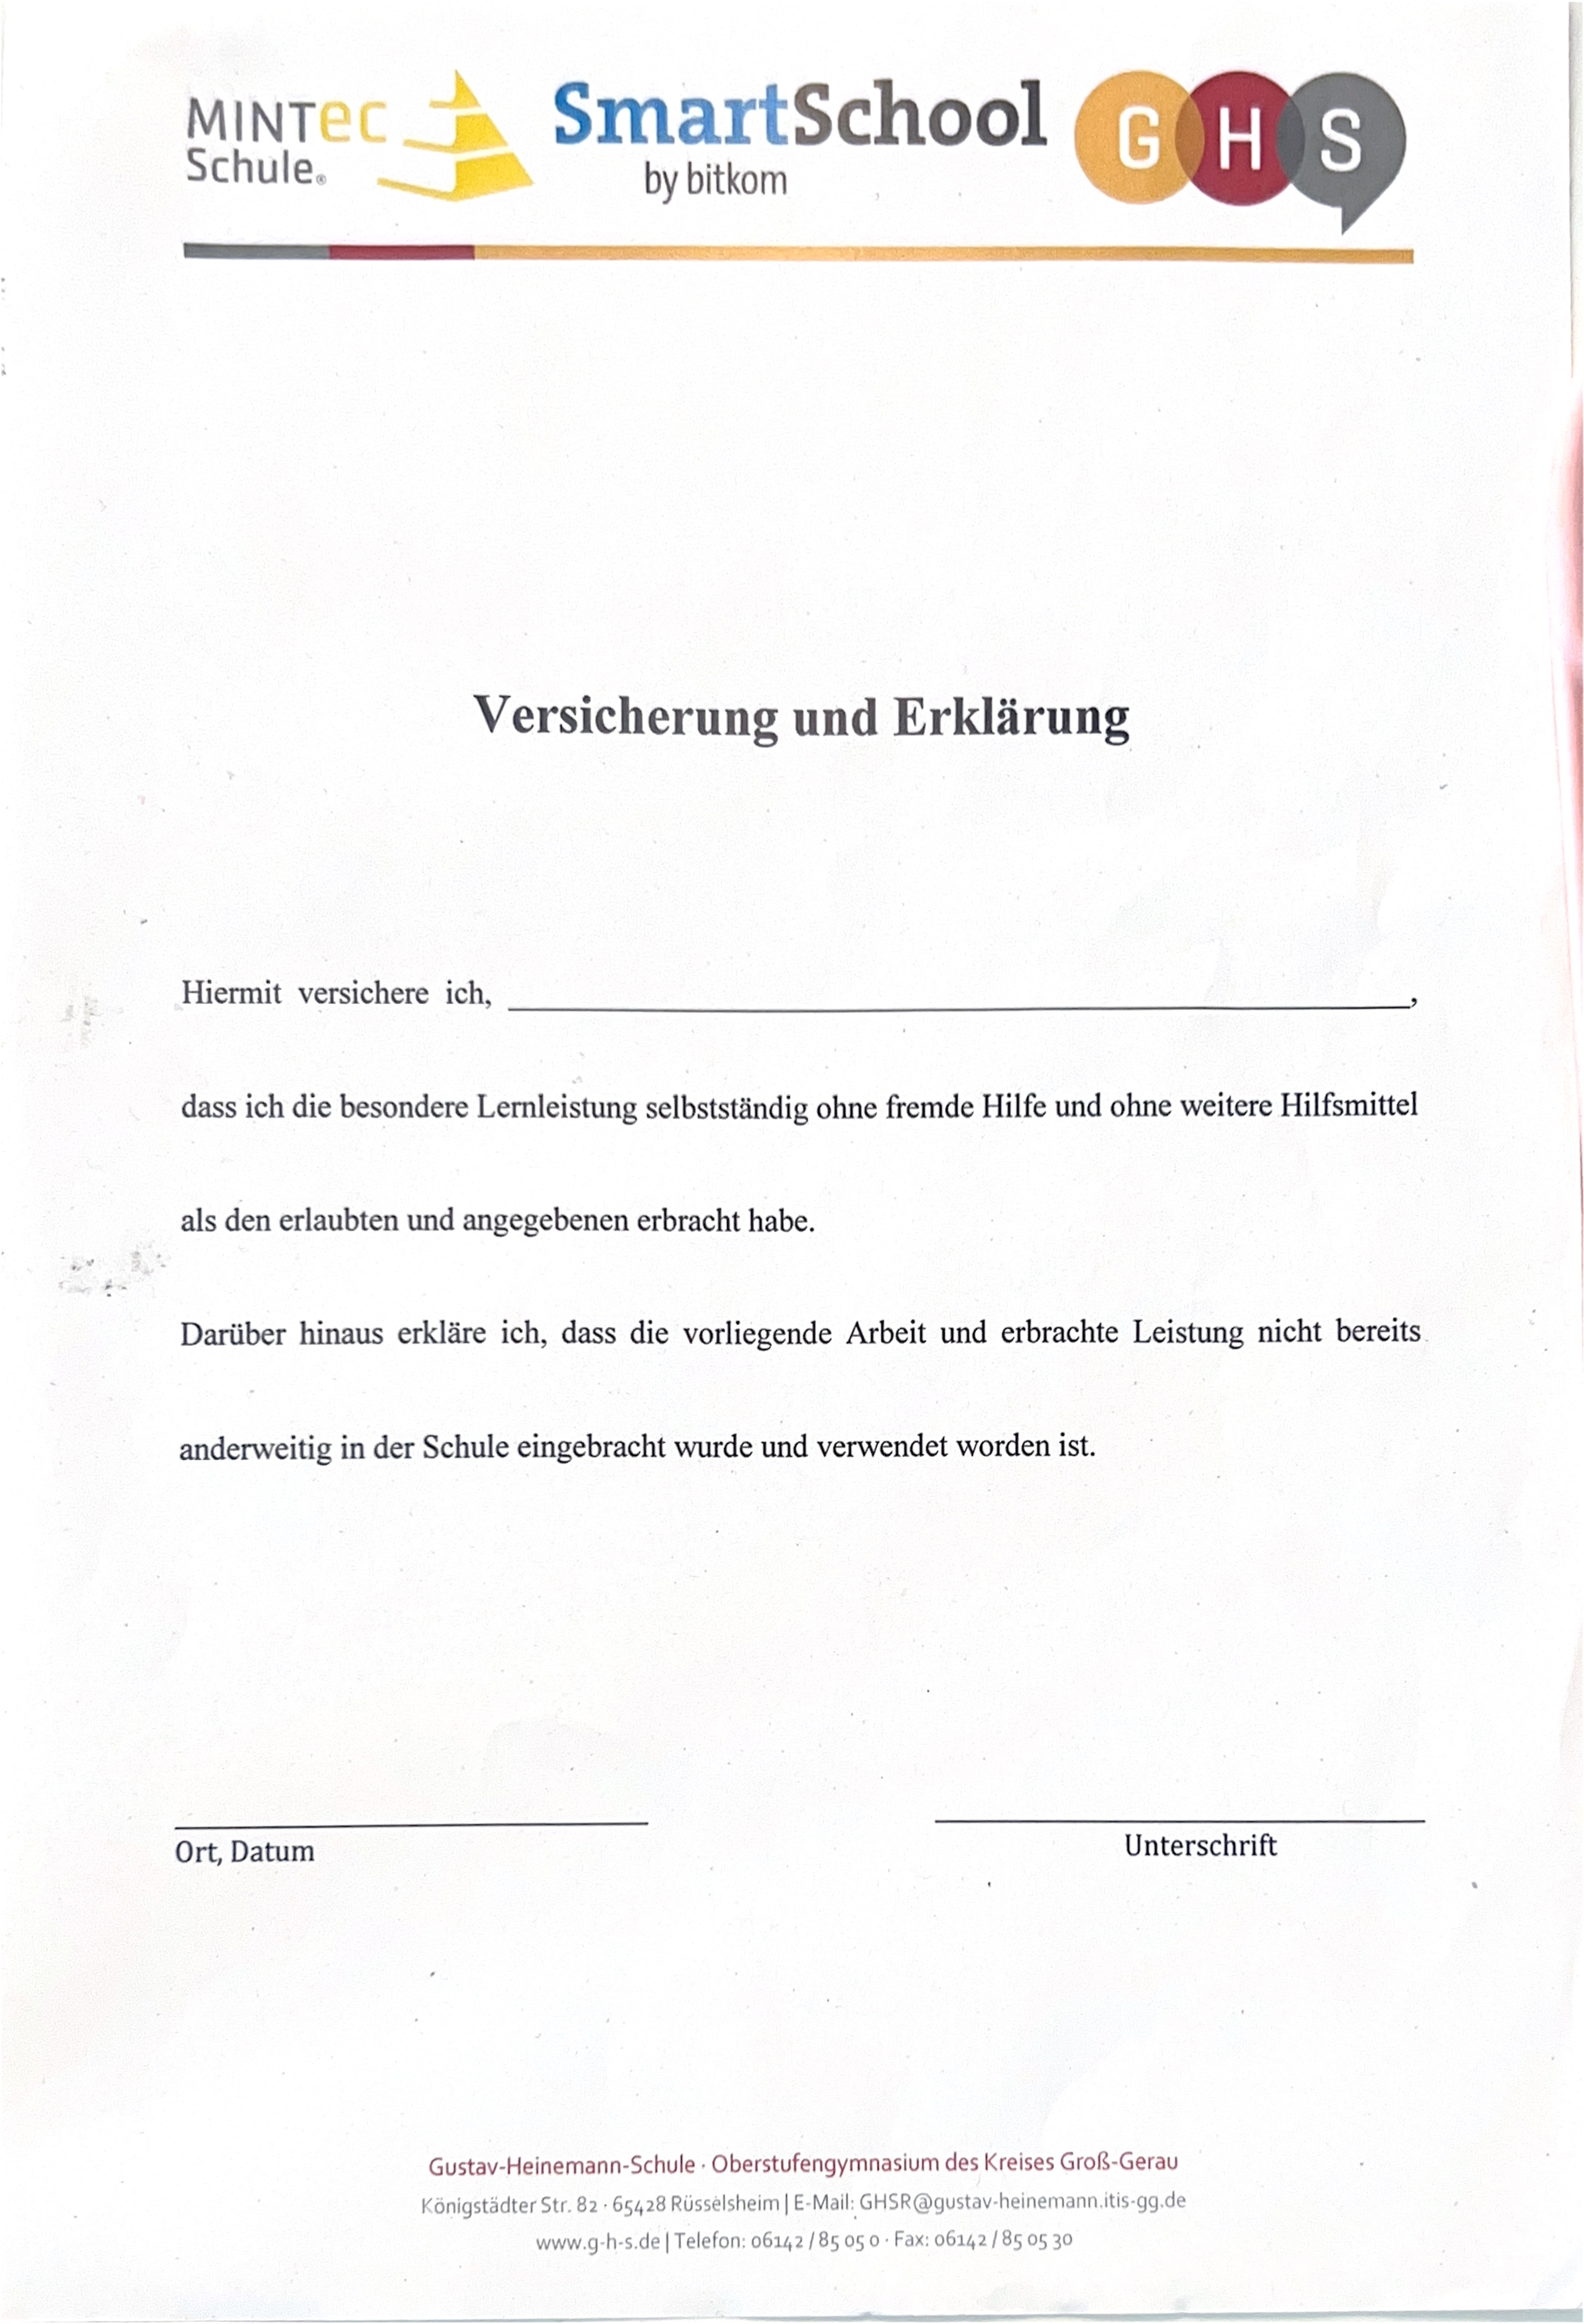
\includegraphics[width= 1.3 \textwidth]{./res/Versicherung.pdf}
     \end{figure}
	\newpage
	\tableofcontents
	\newpage
	
\section{Einleitung}
\label{sec:einleitung}
\subsection{Motivation und Relevanz des Themas}
	Die Verbindung zwischen der physischen und der digitalen Welt spielt eine immer wichtigere Rolle in der modernen Technologieentwicklung. Besonders im Bereich der Mensch-Maschine-Interaktion wird angestrebt, analoge Prozesse effizient zu digitalisieren und in einer computergestützten Umgebung weiterzuverarbeiten. Ein besonders anschauliches Beispiel für ein solches System ist die Digitalisierung analoger Spielzüge im Schach.\\[1ex]
	Schach ist eines der ältesten und zugleich komplexesten Strategiespiele der Menschheitsgeschichte. Während es zahlreiche digitale Schachplattformen gibt, bleibt das klassische Schachbrett mit physischen Figuren für viele Spieler unverzichtbar. Allerdings besteht eine große Herausforderung darin, analoge Schachzüge automatisch und fehlerfrei zu erfassen, um diese für Analysen, Trainingszwecke oder als Schnittstelle für Online-Schachpartien zu nutzen.\\[1ex]
	Hier setzt diese Arbeit an: Durch die Integration von Sensoren in ein physisches Schachbrett sollen Spielzüge erkannt, verarbeitet und digitalisiert werden. Ein solches System könnte nicht nur das Spielerlebnis verbessern, sondern auch wertvolle Funktionen wie Partieverläufe speichern, Fehleranalysen durchführen oder sogar als Trainingshilfe für Schachspieler aller Leistungsstufen dienen.\\[1ex]
	Technisch gesehen ist die Umsetzung einer solchen Mensch-Maschine-Schnittstelle eine interdisziplinäre Herausforderung, da sowohl hardware- als auch softwareseitige Lösungen entwickelt werden müssen. Der Einsatz von Sensorik, Mikrocontrollern und Algorithmen zur Mustererkennung ist daher ein zentraler Bestandteil dieser Arbeit. Zu beachten ist, dass es sich bei dieser Arbeit um einen \glqq\textbf{Proof of Concept}\grqq, also einen exemplarischen Prototyp handelt und ich bei der Entwicklung daher den Schwerpunkt auf die Funktionalität der Schnittstelle gesetzt habe.   
	
	\subsection{Zielsetzung der Arbeit}
	\label{sec:Zielsetzung der Arbeit}
	Das primäre Ziel dieser Arbeit ist die Entwicklung und Implementierung einer Mensch-Maschine-Schnittstelle, die in der Lage ist, analoge Schachzüge automatisch zu erfassen und digital weiterzuverarbeiten. Dazu soll ein Schachbrett mit geeigneten Sensoren ausgestattet werden, um die Positionen der Schachfiguren zu erfassen und ihre Bewegungen zu registrieren.\\[1ex]
	Um dieses Ziel zu erreichen, werden folgende Teilziele verfolgt:
	\begin{itemize}
		\item Entwicklung eines funktionalen Konzepts zur Erfassung der Schachzüge unter Berücksichtigung der technischen Möglichkeiten.
		\item Auswahl geeigneter Sensorik, die eine zuverlässige Identifikation der Figurenpositionen ermöglicht.
		\item Aufbau und Implementierung einer Hardwarelösung, die die Spielzüge in Echtzeit erkennt.
		\item Entwicklung einer Software, die die erfassten Daten interpretiert und eine sinnvolle Ausgabe generiert (z. B. in Form einer digitalen Partienotation oder Schnittstelle zu Schachsoftware).
		\item Test und Evaluierung des entwickelten Systems hinsichtlich Genauigkeit, Zuverlässigkeit und Praxistauglichkeit.
	\end{itemize}
	
	\subsection{Aufbau und Vorgehensweise}
	
	Die Arbeit ist in mehrere Kapitel unterteilt, die die verschiedenen Schritte der Entwicklung systematisch behandeln werden. In folgender Arbeit werde ich daher diese einzelnen Teil Aspekte der Arbeit in Folgende Unterteilen: 
	\begin{enumerate}
	\item \textbf{Theoretische Grundlagen}
	\item \textbf{Entwicklung der Schnittstelle}
	\item \textbf{Umsetzung und Implementierung}
	\item \textbf{Evaluation und Test}
	\item \textbf{Zusammenfassung und Ausblick}
\end{enumerate}

\section{Theoretische Grundlagen}
In diesem Kapitel werden alle technischen, sowie theoretischen Grundlagen vermittelt, die im Vorfeld benötigt werden, um die spätere Methodik der Entwicklung des Projektes erfassen zu können.
\label{sec:theorie}
\subsection{Überblick Mensch-Maschine-Schnittstellen}
	
	Die Benutzerschnittstelle, auch als „Mensch-Maschine-Schnittstelle“ (MMS) bekannt, wird im Englischen als „Human Machine Interface“ (HMI) oder „Man Machine Interface“ (MMI) bezeichnet.\footcite{wikipedia_Benutzerschnittstelle} Sie ermöglicht es dem Nutzer nicht nur, eine Maschine zu steuern, sondern in vielen Fällen auch deren Status zu überwachen und aktiv in den Prozess einzugreifen. Die Rückmeldung („Feedback“) kann dabei auf verschiedene Weise erfolgen: Traditionell geschieht dies über Bedienpulte mit Signallampen, Anzeigefeldern und Tastern. Moderne Systeme setzen hingegen verstärkt auf softwaregestützte Visualisierung, die beispielsweise auf einem Bildschirm oder einem speziellen Terminal dargestellt wird.\footcite{elektrotechnik}\\[1ex]
	Ein Beispiel für eine Mensch-Maschine-Schnittstelle ist eine Mikrowelle. Der Nutzer gibt über Tasten oder ein Touchdisplay die gewünschte Zeit und Leistung ein, woraufhin die Mikrowelle das Essen erwärmt. Das „Feedback“ erfolgt akustisch durch einen Signalton am Ende des Vorgangs sowie visuell durch die Anzeige der verbleibenden Zeit auf dem Display.
	
\subsection{Grundlagen Schach}
	
	Das Schachspiel zählt zu den ältesten Spielen der Welt und hat seinen vermuteten Ursprung im indischen Raum.\footcite{wikipedia_Schachbrett} Es wird auf einem quadratischen Schachbrett gespielt, das üblicherweise in abwechselnd helle und dunkle Felder unterteilt ist (zum Beispiel in hellbraun und dunkelbraun oder schwarz und weiß). Das Brett besteht aus insgesamt 64 Feldern, angeordnet in 8 Spalten, die von 1 bis 8 nummeriert sind, und 8 Reihen, die mit den Buchstaben a bis h bezeichnet werden.\footcite{wikipedia_Schachbrett}\\
	\\
	Im Schach gibt es sechs verschiedene Figuren: den Bauern, den Springer, den Läufer, den Turm, die Dame und den König. Jede Figur besitzt eigene Zugregeln, die festlegen, wie sie sich auf dem Brett bewegen – in der Schachsprache wird dies als „ziehen“ bezeichnet.\\
	\\
	Das Spiel wird von zwei Spielern ausgetragen. Jeder Spieler erhält 16 Figuren, nämlich 8 Bauern, 2 Springer, 2 Läufer, 2 Türme, eine Dame und einen König. Die Figuren werden üblicherweise als schwarz und weiß bezeichnet, wobei die tatsächlichen Farben oft lediglich unterschiedliche Farbtöne (hell bzw. dunkel) sind, um eine Unterscheidung zu ermöglichen.\footcite{Schachbegriffe} Die Spieler ziehen abwechselnd. In jedem Zug kann eine eigene Figur auf dem Spielfeld bewegt werden. Es ist weder möglich, freiwillig auf einen Zug zu verzichten, noch einen bereits getätigten Zug rückgängig zu machen.\footcite{Schachregeln} Figuren der jeweils gegnerischen Farbe können „geschlagen“ werden, das heißt, sie werden aus dem Spiel entfernt. Eine Figur kann nur dann geschlagen werden, wenn sie von einer gegnerischen Figur bedroht wird, also auf einem Feld steht, auf das diese Figur ziehen kann.\footcite{wikipedia_schachfiguren}
	\begin{figure}[H] 
		\centering 
		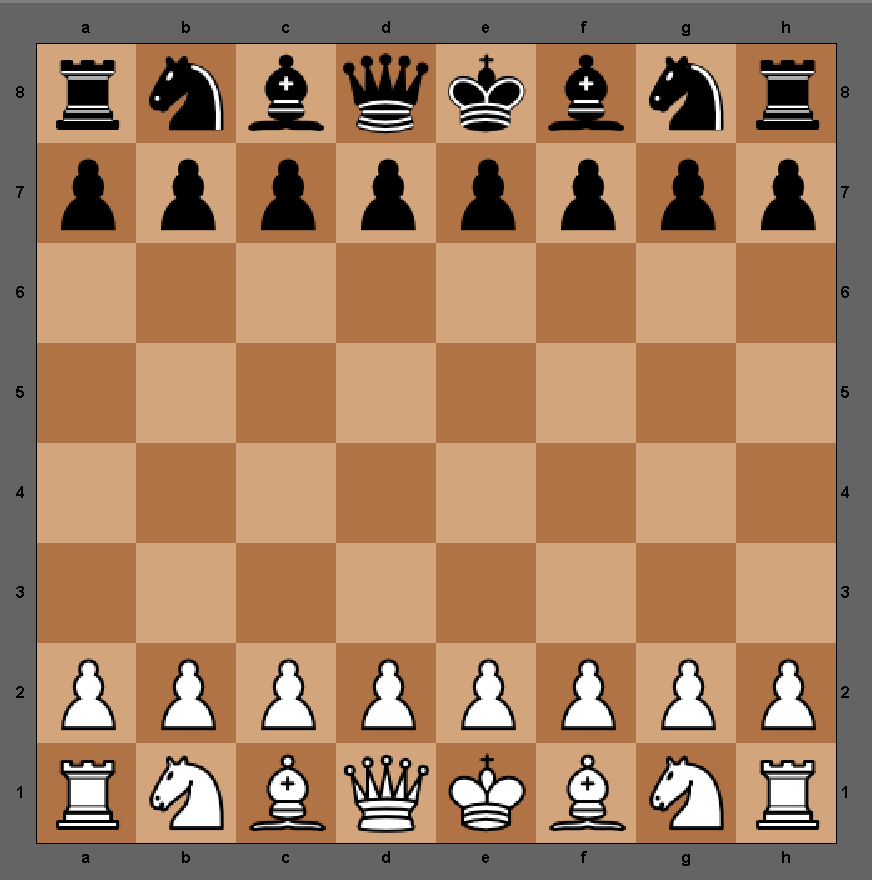
\includegraphics[width=0.5\textwidth]{./res/Schach/Screenshot 2025-03-21 001659.png} 
		\caption{Grundstellung des Schachspiels. (eigens erstellte Abbildung)} \label{fig:Grundstellung des Schachspiels} \end{figure}
	
	Wie in Abbildung \ref{fig:Grundstellung des Schachspiels} dargestellt, ist die Grundaufstellung im Schach folgendermaßen: Die erste und die letzte Reihe werden als „Grund-Reihe“ bezeichnet.\footcite{wikipedia_Schachbrett} Zu Beginn des Spiels befinden sich die Türme auf den Feldern \glqq a1 \grqq und \glqq h1 \grqq, die Springer auf den Feldern b1 und g1, die Läufer auf c1 und f1, die Dame auf d1 sowie der König auf e1 für die weiße Seite. Entsprechend ist die Aufstellung für Schwarz auf der achten Reihe identisch. Die acht Bauern beider Seiten werden jeweils auf der zweiten (für Weiß) und der siebten Reihe (für Schwarz) positioniert.\\
	\\
	Im Schach bewegt sich jede der sechs Figuren auf eine eigene, festgelegte Weise. Dabei gelten folgende Regeln.
	Bauern ziehen grundsätzlich ein Feld geradeaus vorwärts. Beim ersten Zug eines Bauern kann er auch zwei Felder vorgehen, sofern beide frei sind (siehe Abbildung \ref{fig:Bauern_zug}).
	
	\begin{figure}[H]
		\centering
		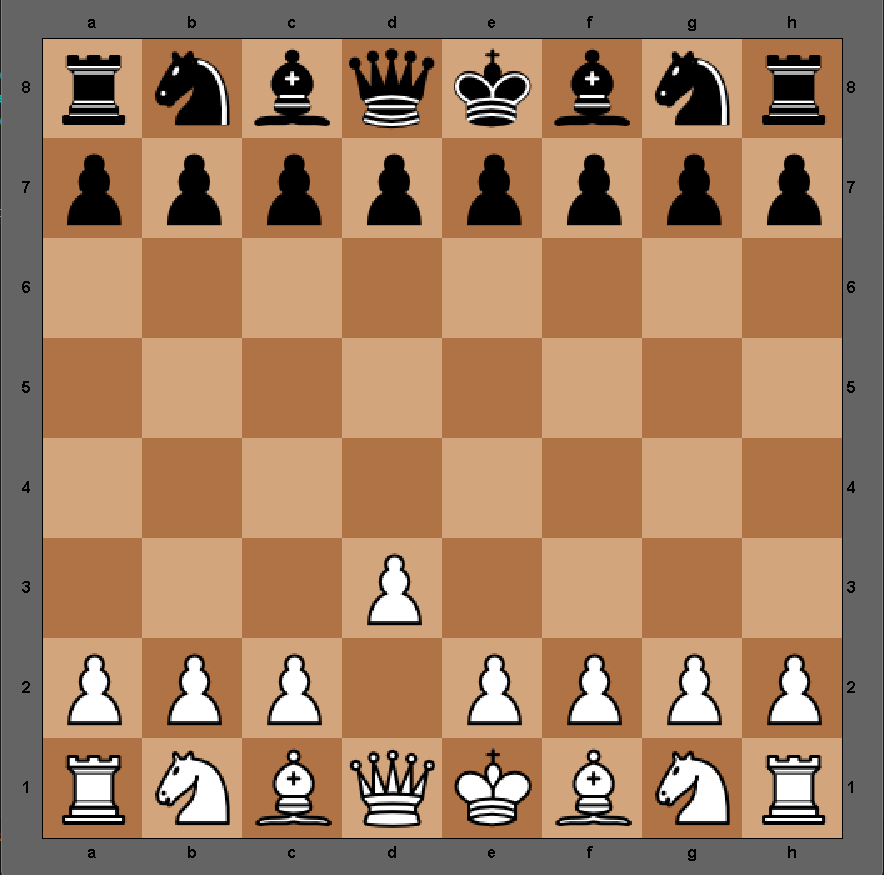
\includegraphics[width=0.4\textwidth]{./res/Schach/Screenshot 2025-03-23 170834.png}
		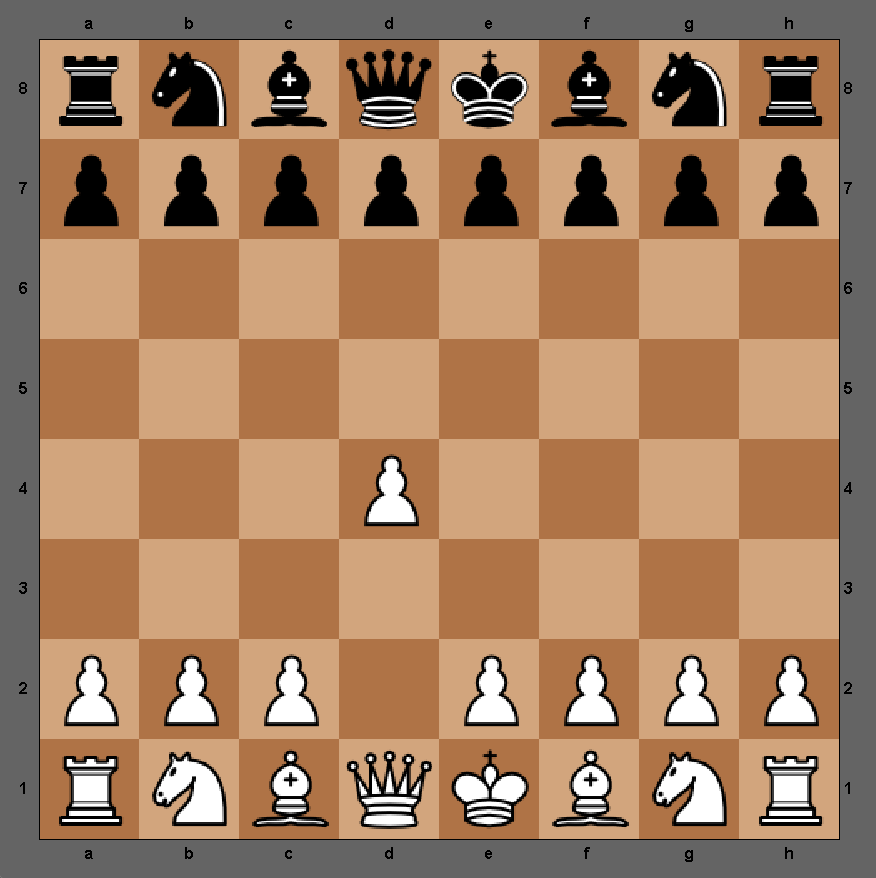
\includegraphics[width=0.4\textwidth]{./res/Schach/Screenshot 2025-03-23 170859.png}
		\caption{Der weiße Bauer zieht von d2 nach d3 und zieht beim erste Zug des Bauern von d2 nach d4. (eigens erstellte Abbildung)}
		\label{fig:Bauern_zug}
	\end{figure}
	

	Erreicht ein Bauer die gegnerische Grundreihe, erfolgt eine Umwandlung (Bauernumwandlung) in eine beliebige andere Figur (außer in den König).\footcite{Schachregeln}\\
	\\
	Der Springer bewegt sich in einem charakteristischen L-förmigen Muster, das heißt zwei Felder in eine Richtung und dann ein Feld rechts oder links davon. Er ist die einzige Figur, die über andere Figuren hinweg springen darf, unabhängig davon, ob diese eigene oder gegnerische Figuren sind.\footcite{Schachregeln}
	
	\begin{figure}[H]
		\centering
		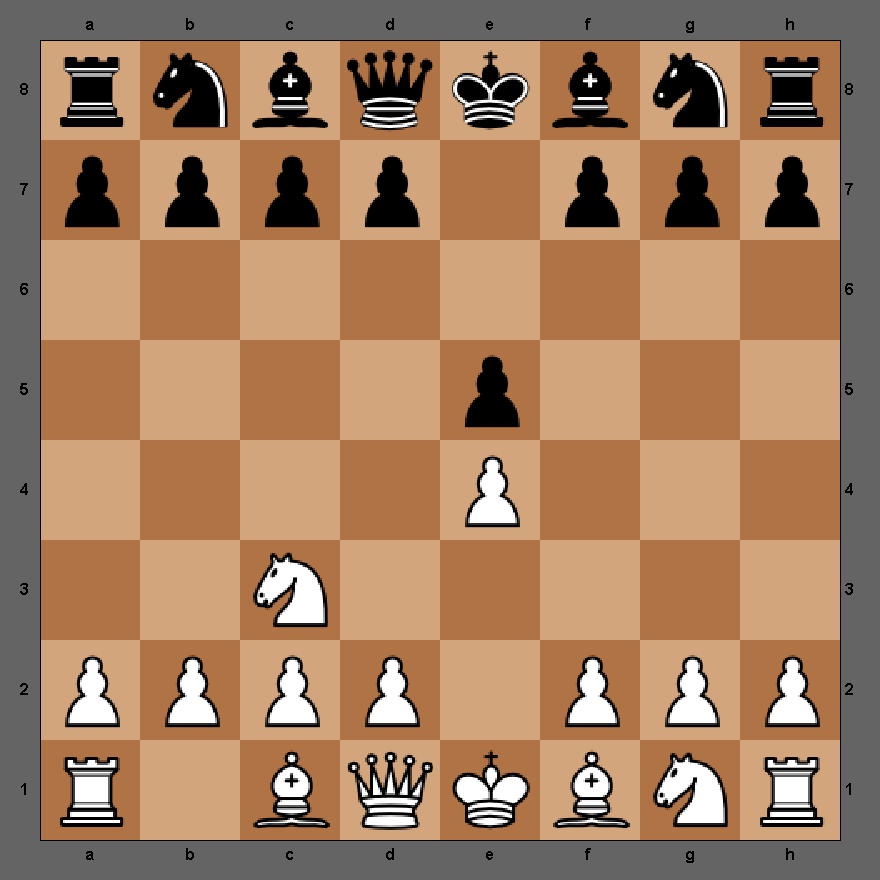
\includegraphics[width=0.5\linewidth]{./res/Schach/beispiel_springer.png}
		\caption{Der weiße Springer zieht von b1 nach c3. (eigens erstellte Abbildung)}
		\label{fig:Beispiel Zug Springer}
	\end{figure}

	Läufer ziehen diagonal über beliebig viele freie Felder und bleiben stets auf Feldern derselben Farbe, wie sie zu Beginn stehen (siehe Abbildung \ref{fig:Beispiel Zug Springer}).\footcite{Schachregeln},
	
	\begin{figure}[H]
		\centering
		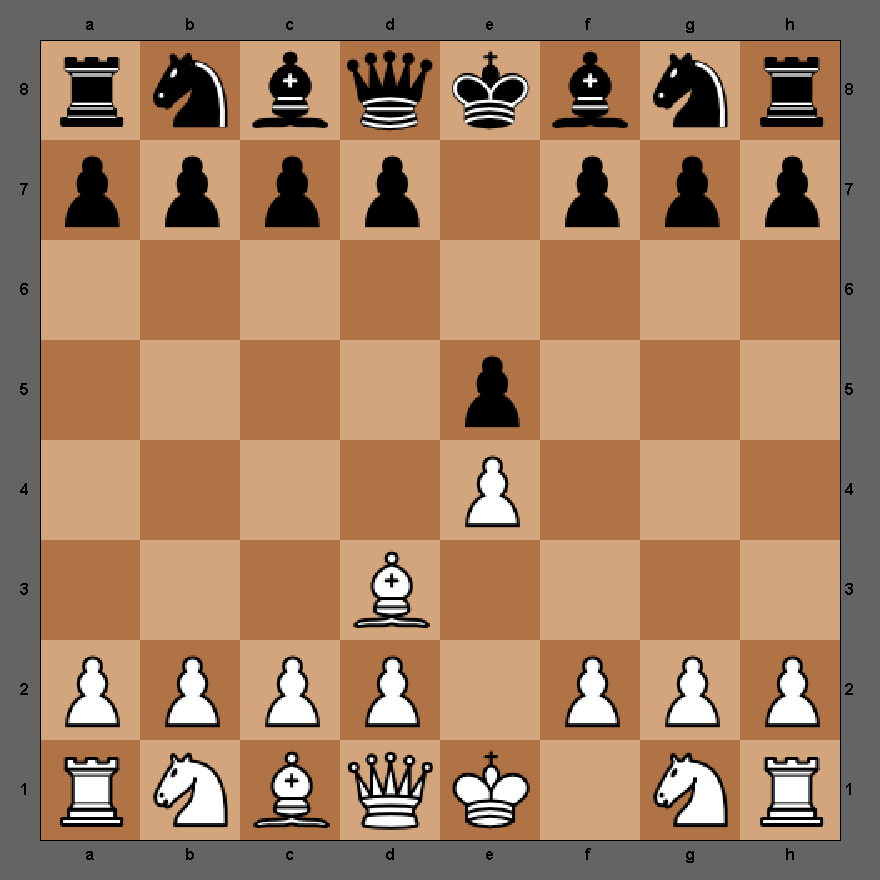
\includegraphics[width=0.5\linewidth]{./res/Schach/Beispielzug_Läufer.png}
		\caption{Der weiße Läufer zieht von f1 nach d3. (eigens erstellte Abbildung)}
		\label{fig:Beispiel Zug Läufer}
	\end{figure}
	
	Türme bewegen sich horizontal oder vertikal über beliebig viele freie Felder (siehe Abbildung \ref{fig:Beispiel_Turm_zug}).\footcite{Schachregeln}
	
	\begin{figure}[H]
		\centering
		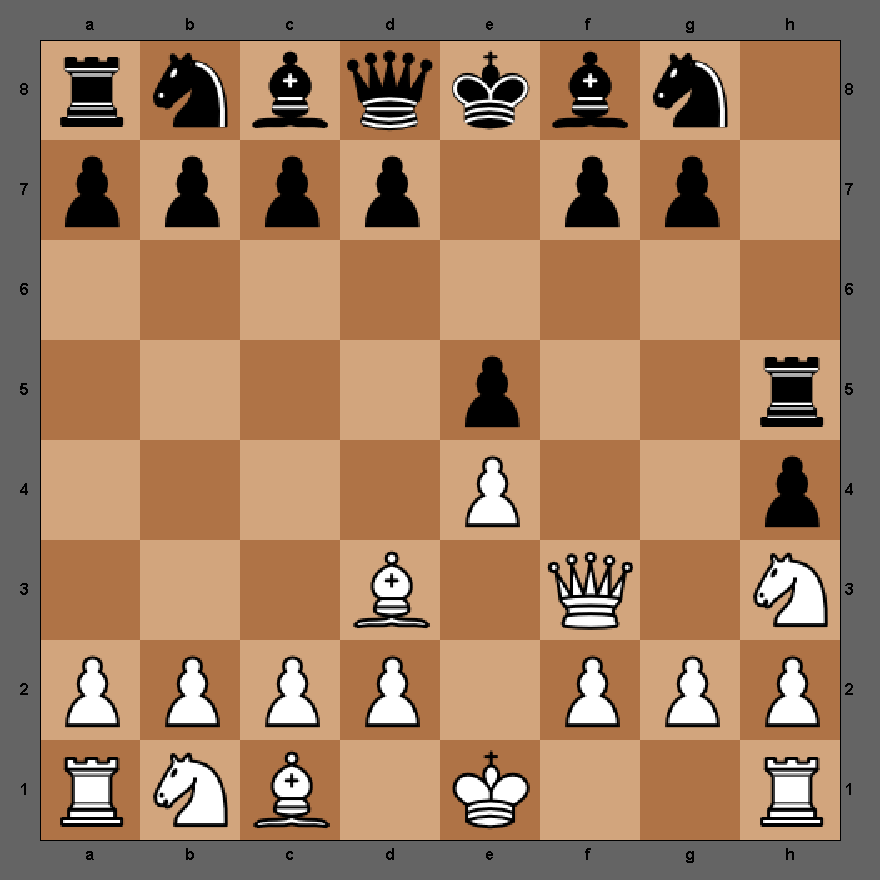
\includegraphics[width=0.5\textwidth]{./res/Schach/BeispielZug_trum.png}
		\caption{Der schwarze Turm zieht von h8 nach h5. (eigens erstellte Abbildung)}
		\label{fig:Beispiel_Turm_zug}
	\end{figure}

	Die Dame kombiniert die Zugmöglichkeiten von Turm und Läufer. Sie kann sich sowohl horizontal, vertikal als auch diagonal über beliebig viele freie Felder bewegen (Siehe Abbildungen \ref{fig:Dame beispielzüge}).\footcite{Schachregeln}
	
	\begin{figure}[H]
		\centering
		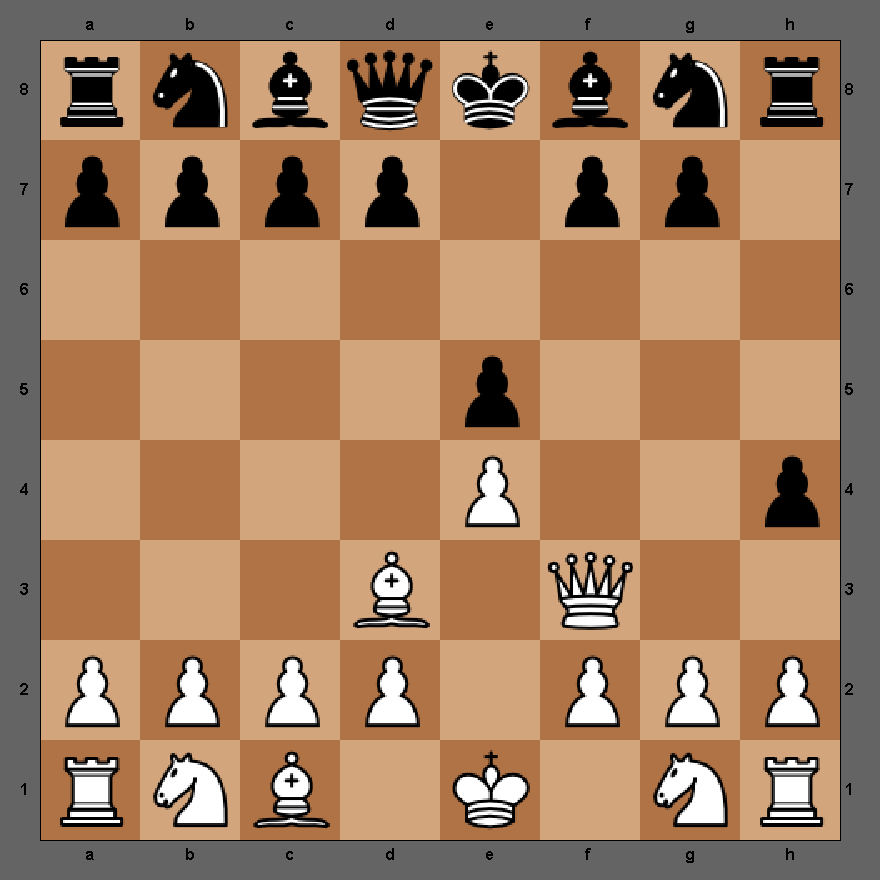
\includegraphics[width=0.4\textwidth]{./res/Schach/Dame_diagnonal.png}
		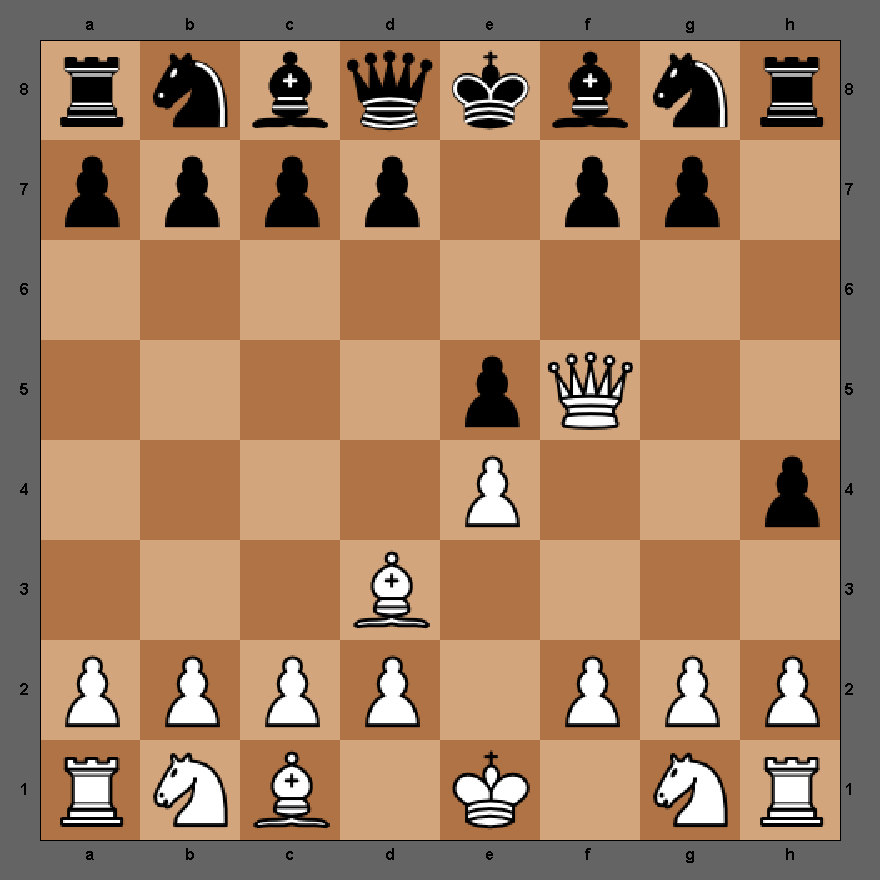
\includegraphics[width=0.4\textwidth]{./res/Schach/Vertikal_dame.png}
		\caption{Die weiße Dame, zieht von d1 nach f3 und weiße Dame, zieht von f3 nach f5. (eigens erstellte Abbildung)}
		\label{fig:Dame beispielzüge}
	\end{figure}
	
	Der König ist die wichtigste Figur im Schachspiel und kann sich in jede Richtung bewegen – sei es horizontal, vertikal oder diagonal –, jedoch stets nur um ein Feld. Dabei ist er besonderen Regeln unterworfen: Er darf kein Feld betreten, das von einer gegnerischen Figur bedroht wird. Gerät der König selbst in Gefahr, also ins Schach, muss der Spieler ihn in diesem Zug aus der Bedrohung befreien.\footcite{Schachbegriffe}\\
	\\
	Eine besondere Bewegung des Königs ist die Rochade, ein Zug, bei dem er gemeinsam mit einem der Türme seine Position verändert. Damit dieser Zug erlaubt ist, müssen mehrere Bedingungen erfüllt sein: Weder der König noch der beteiligte Turm dürfen sich zuvor bewegt haben, zwischen ihnen darf keine andere Figur stehen, und der König darf sich weder im Schach befinden noch während der Rochade ein bedrohtes Feld überqueren oder darauf landen. \footcite{Schachbegriffe}
	
	\begin{figure}[H]
		\centering
		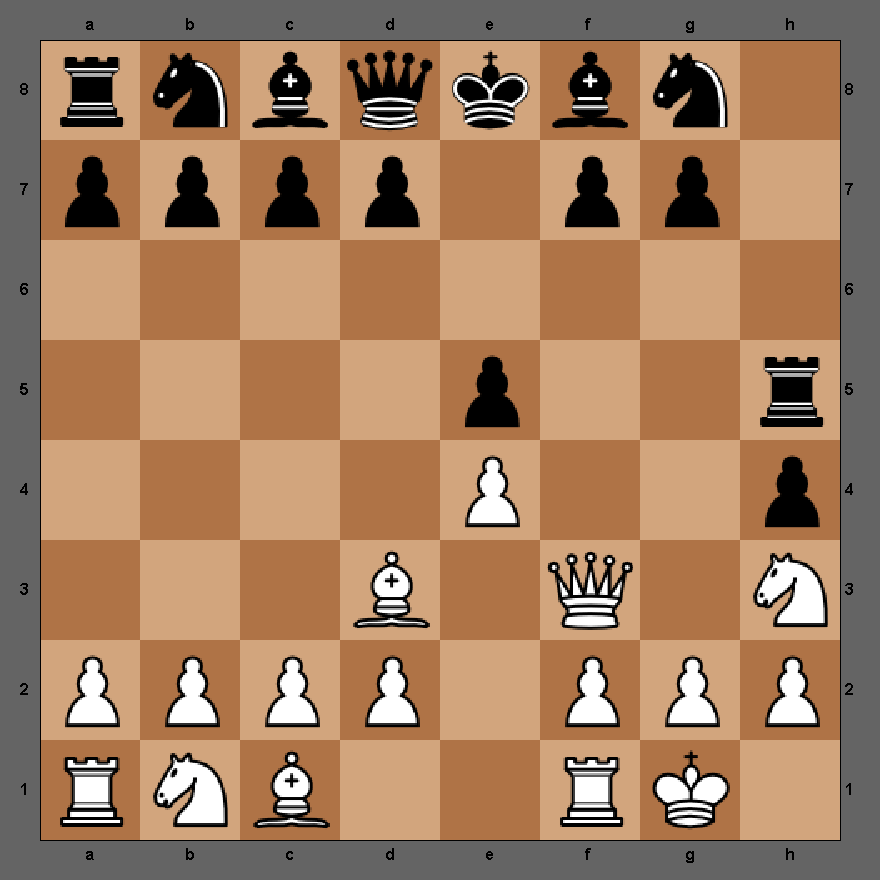
\includegraphics[width=0.4\linewidth]{./res/Schach/Kurze_Rochade.png}
		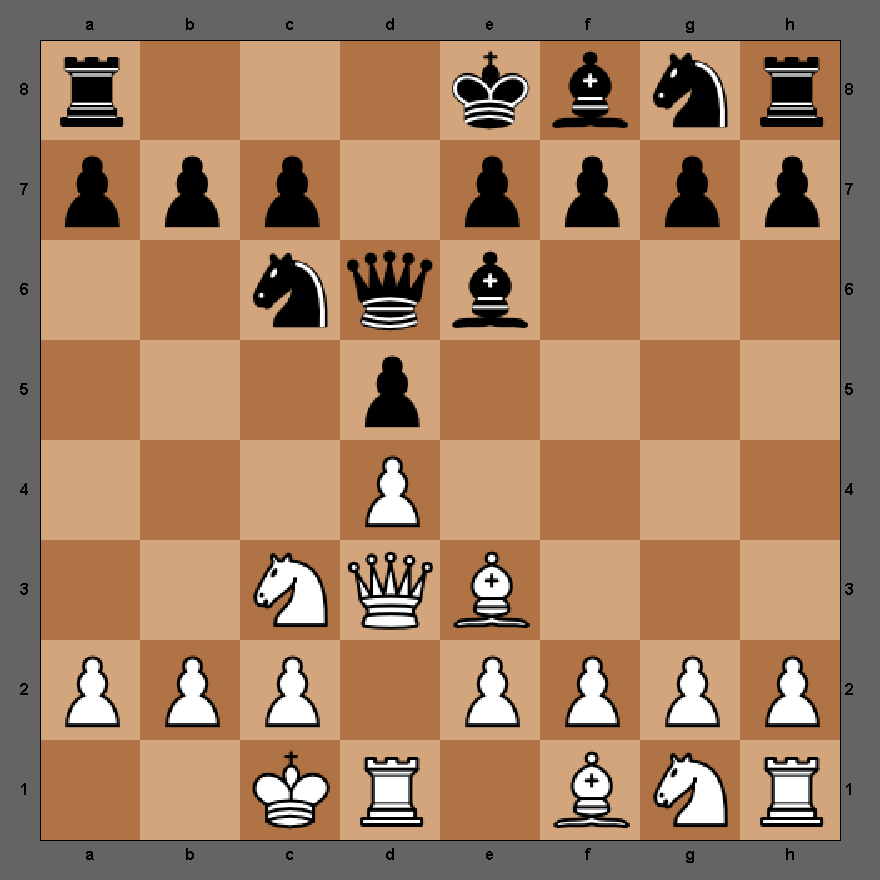
\includegraphics[width=0.4\textwidth]{./res/Schach/Lange_Rochade.png}
		\caption{Lange und kurze Rochade (eigens erstellte Abbildung)}
		\label{fig:enter-label}
	\end{figure}
	
	Mit Ausnahme des Springers kann keine Figur über andere Figuren hinwegziehen. Es ist auch nicht möglich auf ein Feld zu ziehen, welches von einer eigenen Figur besetzt wird. Es ist jedoch erlaubt, auf ein Feld zu ziehen, das von einer gegnerischen Figur belegt ist – in diesem Fall wird die gegnerische Figur geschlagen und aus dem Spiel entfernt. Eine Besonderheit stellt jedoch der Bauer dar. Zum Schlagen zieht der Bauer nämlich ein Feld diagonal vorwärts Staat wie sonst ein Feld geradeaus vorwärts (siehe Abbildung \ref{fig:Bauern_schlagen}).
	
	\begin{figure}[]
		\centering
		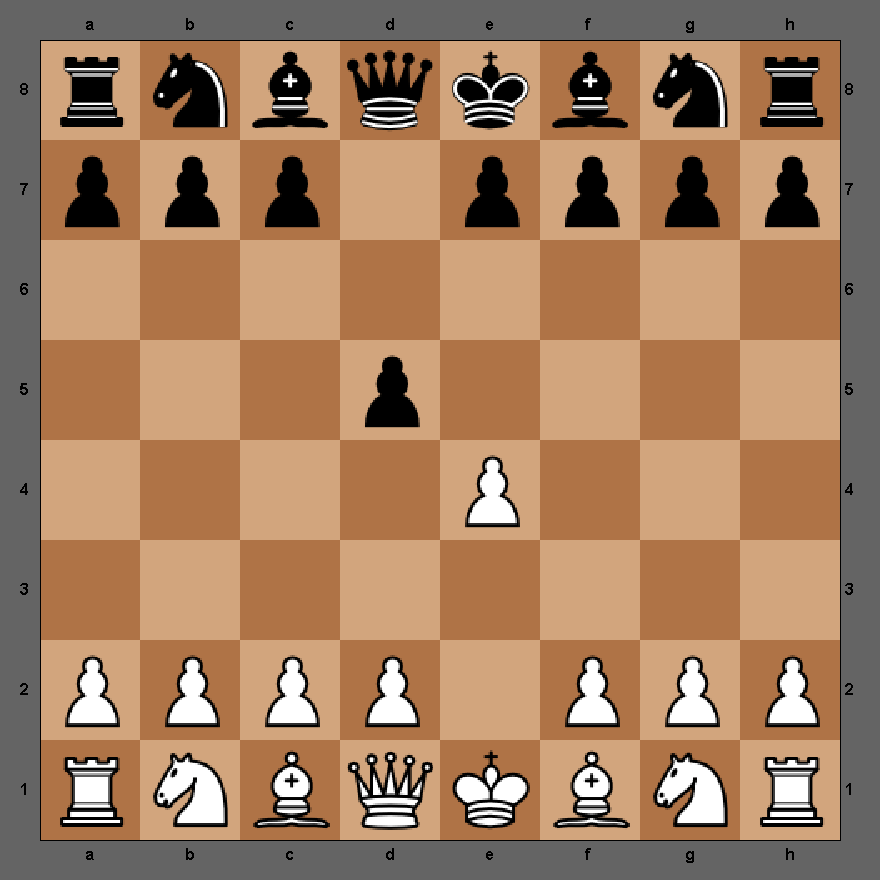
\includegraphics[width=0.4\linewidth]{./res/Schach/Bauern_schlag1.png}
		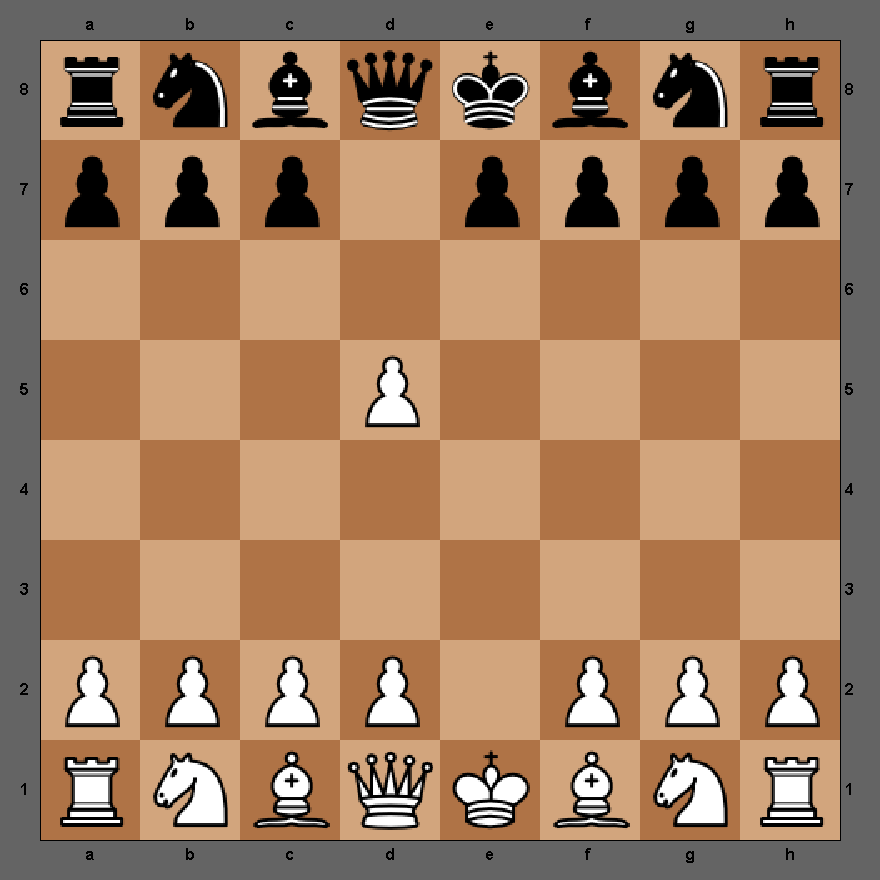
\includegraphics[width=0.4\linewidth]{./res/Schach/BauernSchlag2.png}
		\caption{der weiße Bauer schlägt Schwarz auf Diagonal auf d5. (eigens erstellte Abbildung)}
		\label{fig:Bauern_schlagen}
	\end{figure}
	Zudem gibt es die \textbf{En Passant}-Regel, zu deutsch \glqq\textbf{im Vorübergehen}\grqq. Diese gilt, wenn ein Bauer einen Doppelschritt macht und neben einem gegnerischen Bauern steht, dann kann dieser Bauer hinter den gegnerischen Bauern Ziehen und dabei schlagen (siehe Abbildung \ref{fig:en-passant}). \footcite{Schachregeln}
	
	\begin{figure}[H]
		\centering
		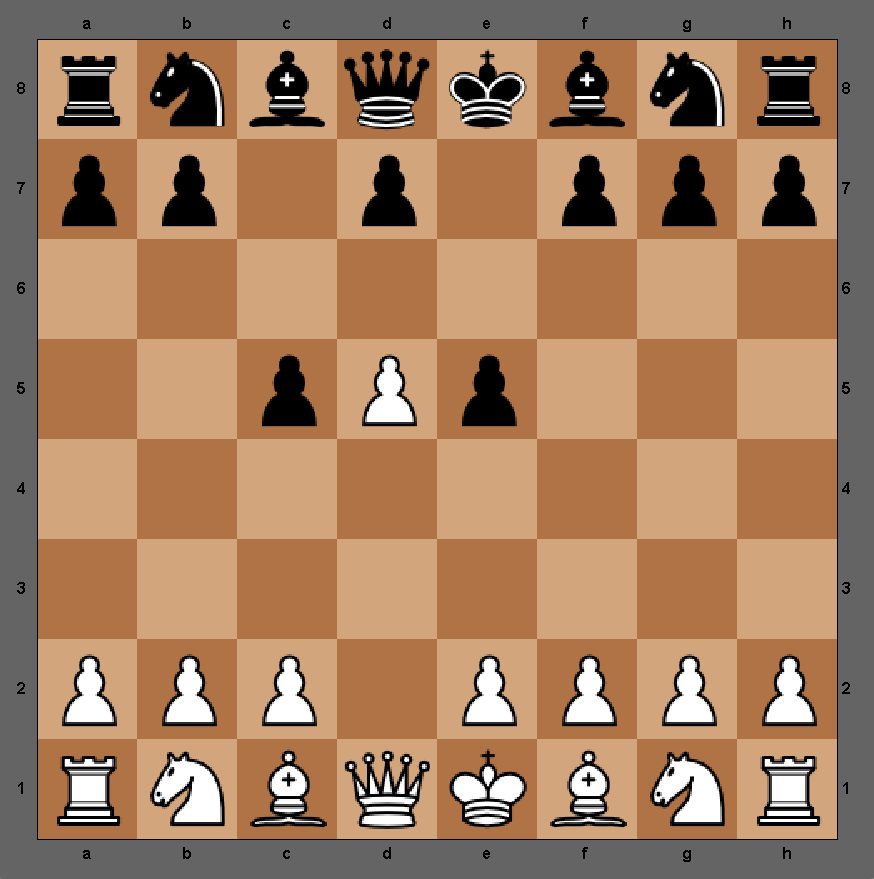
\includegraphics[width=0.4\textwidth]{./res/Schach/En-passant.png}
		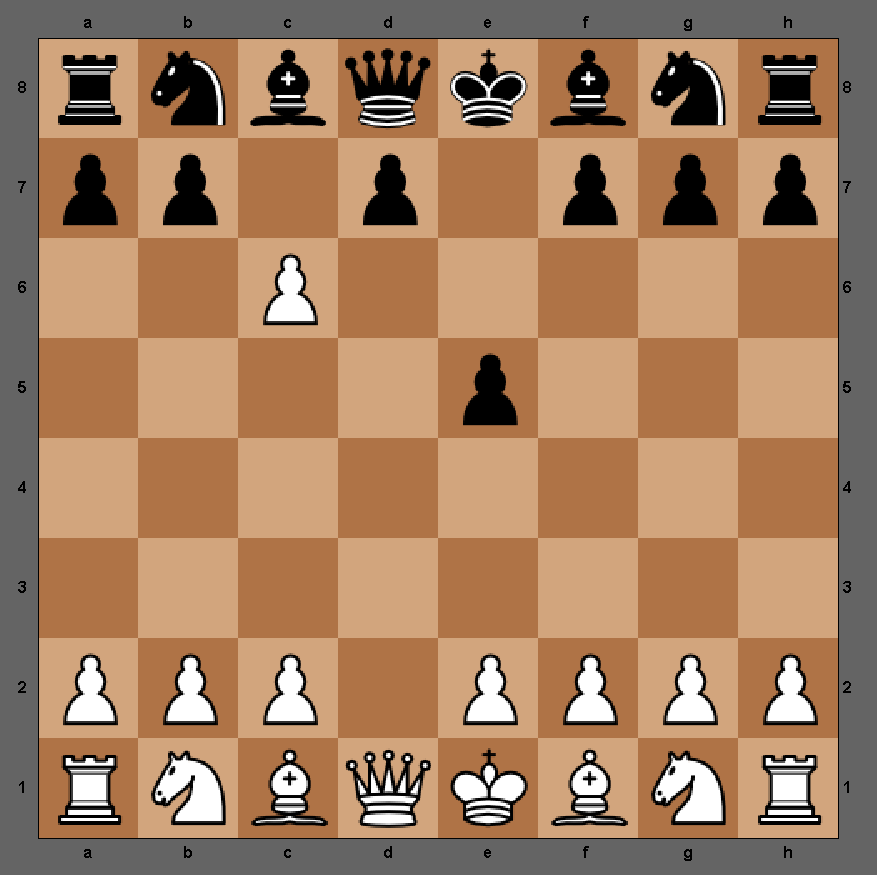
\includegraphics[width=0.4\textwidth]{./res/Schach/En-passant-geschlagen.png}
		\caption{Beispielstellung für En Passant: Der weiße Bauer schlägt den schwarzen Bauern auf c5 im Vorübergehen. (eigens erstellte Abbildung)}
		\label{fig:en-passant}
	\end{figure}
	Darüber hinaus besitzt die weiße Seite den \glqq\textbf{Anzugsvorteil}\grqq, was bedeutet, dass Weiß den ersten Zug ausführen darf und somit von Beginn an die Initiative übernimmt.\footcite{wikipedia_schachspiel}\\
	\\
	Das Ziel des Spiels besteht darin, den gegnerischen König in ein sogenanntes „\textbf{Schachmatt}“ \footcite{Schachregeln} zu setzen. Dies bedeutet, dass der König angegriffen wird (im „Schach“ steht) und keine Möglichkeit hat, der Bedrohung durch Ausweichen, Schlagen der angreifenden Figur oder Decken des Königs durch eine eigene Figur zu entkommen. Wer den gegnerischen König Schachmatt setzt, gewinnt die Partie.\footcite{wikipedia_schachspiel} Eine Partie kann auch im Unentschieden oder auch \glqq \textbf{remis}\grqq \space Enden, wenn z.B 50 Züge lange weder ein Bauer gespielt wurde noch eine Figur geschlagen wurde, oder aber ein Schachmatt nicht mehr möglich ist, Zwei König sind nur noch auf dem Feld übrig.  
%%%%
%
%
% ELEKRONISCHE KOMPONENETEN
%
%%%%%
\subsection{Elektronische Komponenten}
Für die Sensorik kamen bei der Auswahl des Projekts viele verschiedene Bauteile in Betracht. Im Folgenden werden die zentralen Komponenten detailliert erläutert, ihre Funktionsweise beschrieben und durch Schaubilder visualisiert. Zu diesen Komponenten zählen unter anderem die Hallsensoren, der Multiplexer und der Arduino Mega.\\
\\
Ein \textbf{Mikrocontroller} ist ein kompakter integrierter Schaltkreis, der alle Komponenten eines minimalen Computersystems vereint: Einen Prozessor (CPU), programmierbaren Speicher (Flash/ROM) sowie konfigurierbare Ein- und Ausgänge (I/O-Pins). Im Gegensatz zu Mikroprozessoren benötigen Mikrocontroller keine externen Komponenten für den Betrieb und sind speziell für Steuerungs- und Regelungsaufgaben optimiert. Sie werden in eingebetteten Systemen eingesetzt, wo sie Sensordaten erfassen, verarbeiten und darauf basierend z.B Motoren oder LEDs ansteuern.\\
\\
Der \textbf{Arduino Mega rev 3} ist eine Mikrocontroller-Platine, die auf dem \textbf{ATmega2560}-Chip basiert. Als programmierbare Steuereinheit kombiniert er Rechenleistung, Speicher und anpassbare Ein-/Ausgänge in einem kompakten System. Mit einer Taktfrequenz von \SI{16}{\mega\hertz}, \textbf{54 digitalen I/O-Pins} und \textbf{16 analogen Eingängen} eignet er sich besonders für Echtzeit-Anwendungen wie die Sensordatenverarbeitung in diesem Projekt. In Abbildung \ref{fig:arduino_mega_schema} ist eine schematische Darstellung des Arduino Mega rev 3 zu sehen.
\begin{figure}[H]
	\centering
	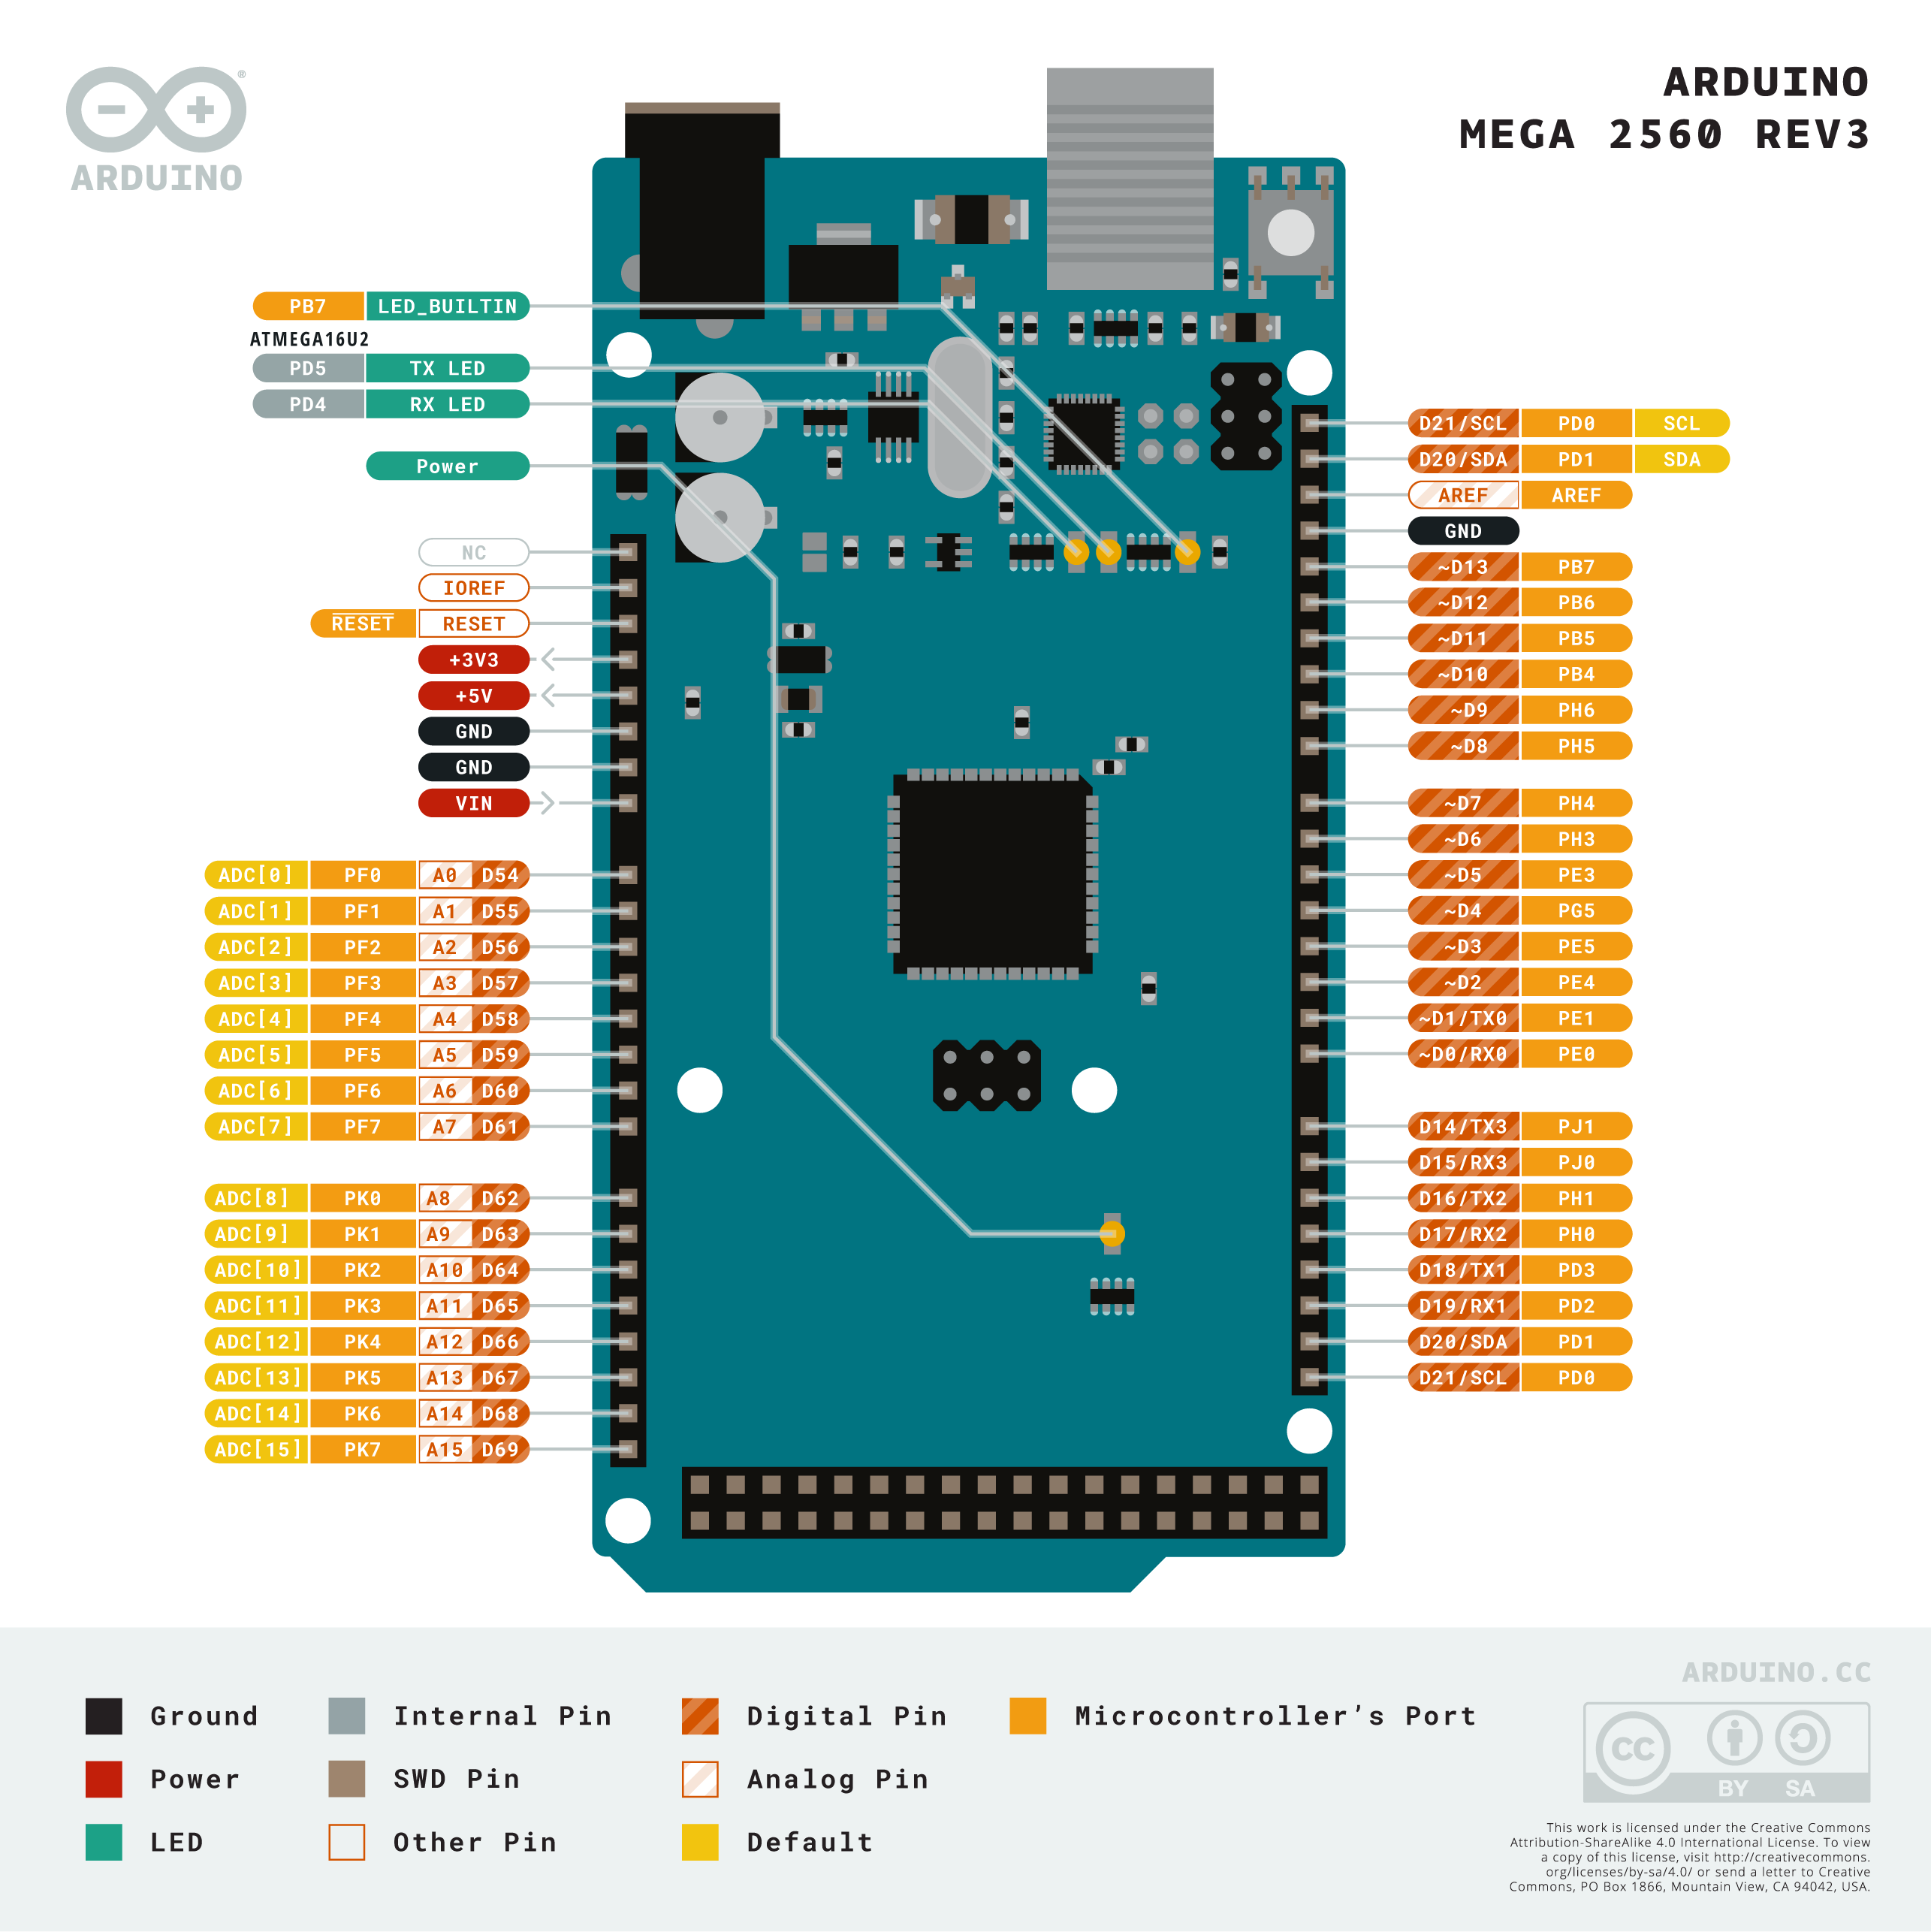
\includegraphics[width=0.40\textwidth]{./res/Elektronik/Pinout-Mega2560rev3_latest.png}
	\caption{Übersicht der Arduino Mega-Platine mit den wichtigsten Anschlüssen \cite{Arduino_Mega}.}
	\label{fig:arduino_mega_schema}
\end{figure}

Die im Projekt zur primären Erfassung eingesetzten \textbf{Hallsensoren} basieren auf dem \textbf{Hall-Effekt}. Wird ein stromdurchflossener Leiter in ein homogenes Magnetfeld gebracht, wirkt auf die beweglichen Elektronen die Lorentz-Kraft. Diese bewirkt, dass sich die Elektronen seitlich sammeln, sodass an den gegenüberliegenden Seiten des Leiters ein Ladungsungleichgewicht entsteht. Dieses Ungleichgewicht erzeugt ein internes elektrisches Feld, das sich so lange aufbaut, bis die Kraft des elektrischen Feldes die Lorentz-Kraft ausgleicht. Das Ergebnis ist eine messbare Spannung, die Hall-Spannung \(U_{\rm{H}}\), welche sich senkrecht zur Strom- und Magnetfeldrichtung befindet. Mathematisch lässt sich die Hall-Spannung folgendermaßen ausdrücken:
\[
U_{\rm{H}} = R_{\rm{H}} \cdot \frac{I \cdot B}{d},
\]
Diese Eigenschaft wird genutzt, um Magnetfelder präzise zu messen.\footcite{Hallsensoren_physik} Im speziellen Fall der eingesetzten digitalen unipolaren Hallsensoren reagiert das Bauteil ausschließlich auf Magnetfelder einer bestimmten Polarität, beispielsweise nur auf den Nordpol. Sobald der Magnetfeldstärke-Schwellwert überschritten wird, ändert der Sensor seinen Ausgangszustand von HIGH zu LOW oder umgekehrt. Dadurch entsteht ein klar abgegrenztes digitales Signal, das direkt von einem Mikrocontroller ausgelesen werden kann. Ein schematischer Aufbau eines solchen Sensors ist in Abbildung \ref{fig:hallsensor_schematisch} dargestellt.
\\
\begin{figure}[H]
	\centering
	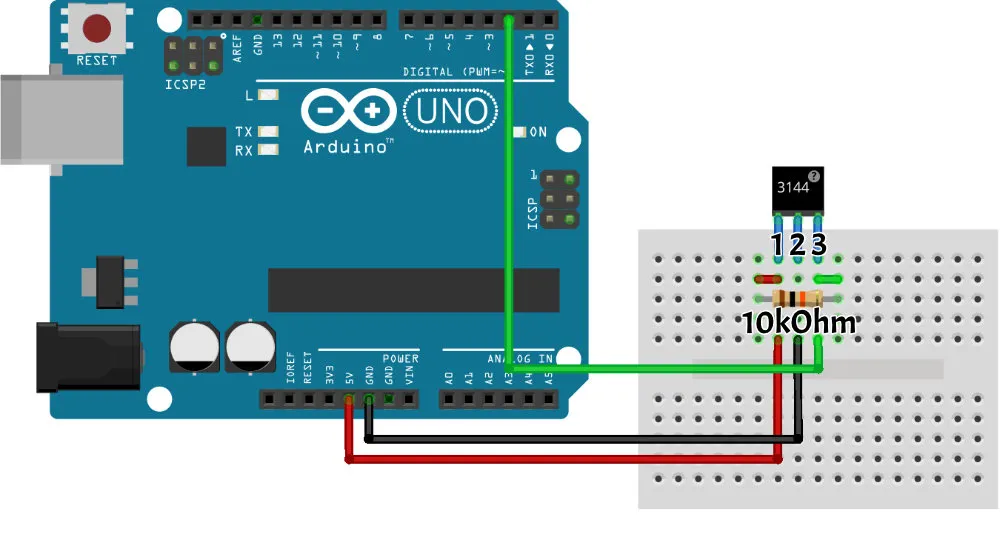
\includegraphics[width=0.7\textwidth]{./res/Elektronik/3144_Hall_Effect_Sensor.png}
	\caption{Schematische Darstellung eines digitalen unipolaren Hallsensors. Quelle: \cite{Hallsensoren_Arduino_projekt}}
	\label{fig:hallsensor_schematisch}
\end{figure}

In Anwendungen, in denen viele Sensoren verwendet werden, ist es oft unpraktisch, jeden Sensor direkt an den Mikrocontroller anzuschließen, da die Anzahl der verfügbaren Ein- und Ausgänge begrenzt ist. Ein \textbf{Multiplexer (MUX)} löst dieses Problem, indem er 16 Eingangssignale sequenziell über einen gemeinsamen Ausgang ausgibt. Dafür werden vier Adressleitungen (\(S_0\) bis \(S_3\)) benötigt, da \(2^4 = 16\) mögliche Kombinationen existieren. Ein 4-Bit-Steuercode legt fest, welcher der 16 Kanäle (\(C_0\) bis \(C_{15}\)) aktiviert wird. Dies reduziert den Anschlussaufwand erheblich, da nur ein Ausgangssignal (SIG) und vier Steuerleitungen erforderlich sind.

\begin{figure}[H]
	\centering
	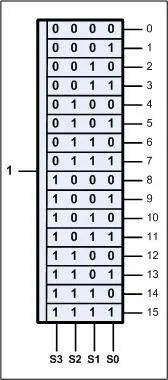
\includegraphics[width=0.2\textwidth, height = 0.21 \textheight]{./res/mux_16_bas.png}
	\caption{Adresstabelle des 16:1-Multiplexers. Die vier Adressbits (\(S_3\) bis \(S_0\)) bestimmen den aktiven Kanal \(C_0\) bis \(C_{15}\),     \cite{Mux_tablle}}
	\label{fig:mux_table}
\end{figure}

Der \textbf{CD74HC4067} ist ein typischer 16:1-Multiplexer für Mikrocontroller-Anwendungen. Die Tabelle in Abbildung \ref{fig:mux_table} zeigt die Zuordnung zwischen dem 4-Bit-Code und den Kanälen. Beispielsweise wird Kanal \(C_9\) aktiviert, wenn \(S_3 = 1\), \(S_2 = 0\), \(S_1 = 0\), und \(S_0 = 1\) (Binärcode \texttt{1001}). Der \textbf{SIG}-Pin gibt dann das Signal des Sensors an \(C_9\) aus. Der \textbf{EN}-Pin (\textit{Enable}) steuert die Aktivierung des Multiplexers: Bei \textbf{GND}-Pegel ist das Modul aktiv, bei \textbf{VCC} deaktiviert.

\begin{figure}[H]
	\centering
	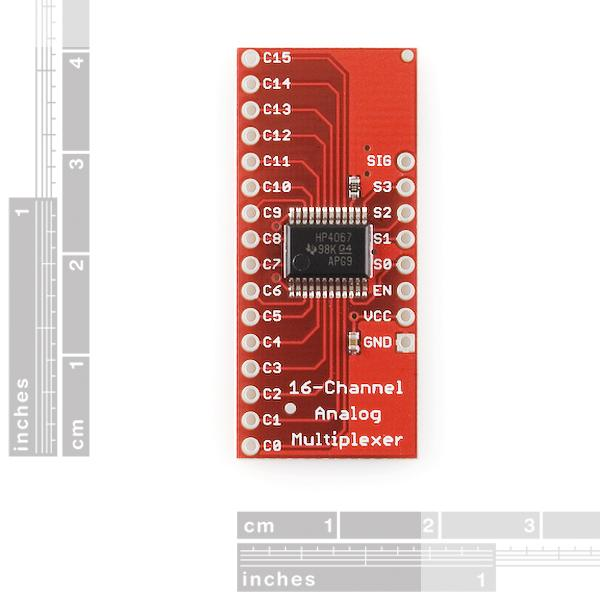
\includegraphics[width=0.5\textwidth]{./res/Elektronik/MUX_Schema.jpg}
	\caption{Schaltplan des 16:1-Multiplexers CD74HC406, \cite{Analog_Digital_MUX}}
	\label{fig:mux_schema}
\end{figure}
%%%%
% Entwicklung der Schnittstelle
%%%%%
\section{Entwicklung der Schnittstelle}
\subsection{Grundideen und Konzepte}
Die Entwicklung der Schnittstelle begann mit der Auswahl eines geeigneten physischen Schachbretts als Grundlage. Ich entschied mich für ein klassisches Holzschachbrett, da es nicht nur stabil, sondern auch ästhetisch ansprechend war.„Um einen besseren Eindruck vom verwendeten Schachbrett zu vermitteln, ist in Abbildung~\ref{fig:schachbrett} eine Darstellung zu sehen. Damit es jedoch als digitale Schnittstelle dienen konnte, musste es mit Sensoren ausgestattet werden, die die Positionen der Figuren erfassen konnten.“

\begin{figure}[H]
	\centering
	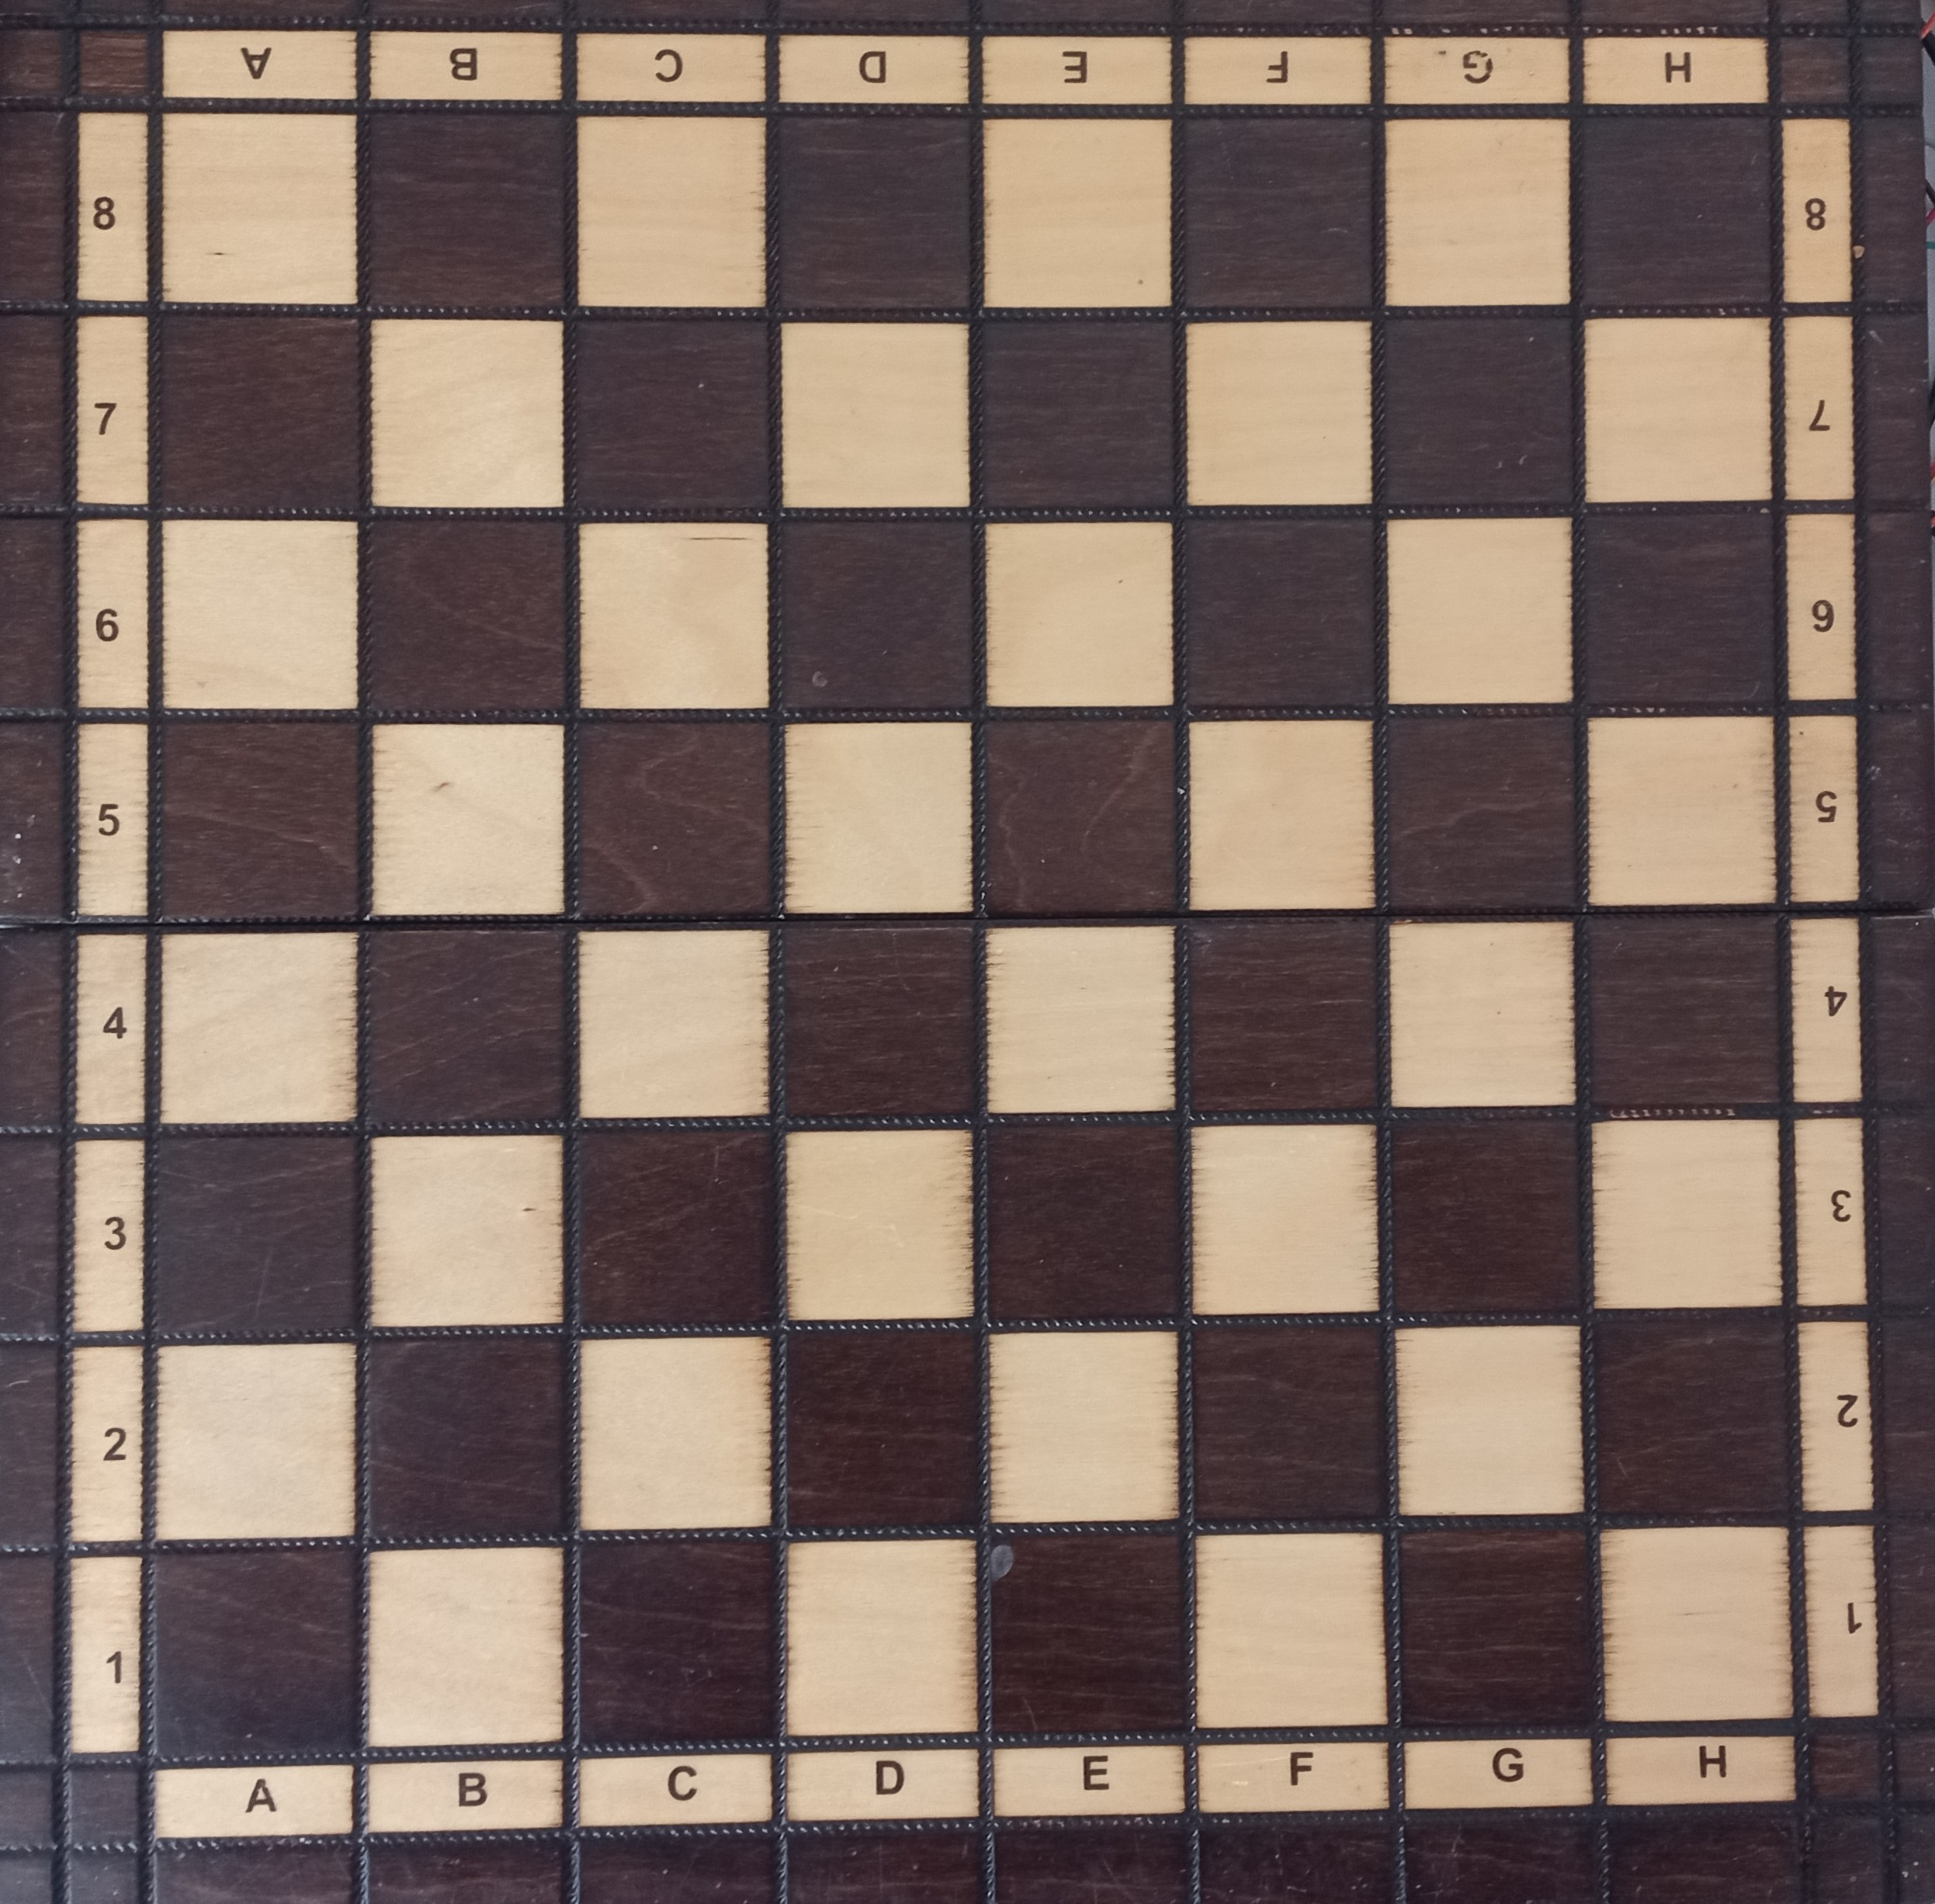
\includegraphics[width=0.5\textwidth, height= 0.15 \textheight]{./res/Schach/Schachbrettv1.jpg}
	\caption{Ein herkömmlichen Holzschachbrett, das als Basis für die Schnittstellenentwicklung gewählt wurde.}
	\label{fig:schachbrett}
\end{figure}
Mein Konzept sah vor, das Schachbrett durch eine eigens vorgenommene Verkabelung mit Sensoren auszustatten. Dafür platzierte ich unter jedem der 64 Felder gezielt eine Lücke in der Kupferkabelmatrix. An diesen definierten Stellen entfernte ich die Isolierung der Leitungen und lötete jeweils einen Sensor an.\\
\\
Die Wahl der Hallsensoren war das Ergebnis einer Abwägung verschiedener Technologien. Ursprünglich hatte ich auch an RFID-Scanner gedacht, da sie die Möglichkeit geboten hätten, nicht nur die Positionen, sondern auch die Identität der Figuren zu erkennen. Allerdings hätten RFID-Scanner ein erhebliches Platzproblem mit sich gebracht. Jeder Scanner benötigt eine gewisse Fläche, und die gegenseitige Beeinflussung der Scanner durch Interferenzen auf engstem Raum hätte es nahezu unmöglich gemacht, verlässliche Messungen durchzuführen~\footcite{Rfid}.\\
\\
Hallsensoren hingegen boten eine einfachere und kompaktere Lösung. Sie messen magnetische Felder, was bedeutete, dass jede Figur lediglich mit einem kleinen Magneten in der Basis ausgestattet werden musste, um von den Sensoren erkannt zu werden. Diese Lösung war platzsparend und technisch leicht umsetzbar. Ein entscheidender Nachteil dieser Methode war jedoch, dass die Sensoren lediglich das Vorhandensein einer Figur auf einem bestimmten Feld erkennen konnten, nicht jedoch die Identität der Figur selbst. Während RFID-Scanner theoretisch in der Lage gewesen wären, zwischen König, Dame oder Bauer zu unterscheiden, war dies mit Hallsensoren nicht ohne Weiteres möglich. Dieses Problem sollte später noch eine Herausforderung darstellen, insbesondere bei der genauen Rekonstruktion von Spielzügen~\footcite{reddit_schachbrett}.\\
\\
Um die fehlende Unterscheidbarkeit der Figuren zumindest im Spiel zu kompensieren, suchte ich aus dem Internet nach einem 3D-Modell für Schachfiguren.\footcite{3D_Figuren} Ich passte dieses Modell so an, dass Magneten an den Figuren befestigt werden konnten. Diese angepassten Schachfiguren sollen dann als echte Spielfiguren verwendet werden.\\
\begin{figure}[H]
	\centering
	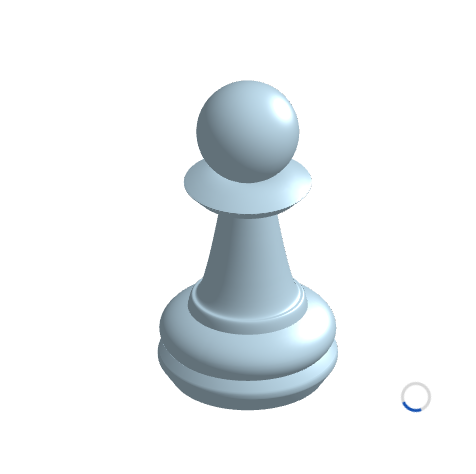
\includegraphics[width=0.15\textwidth]{./res/Schach/3D_Bauer}
	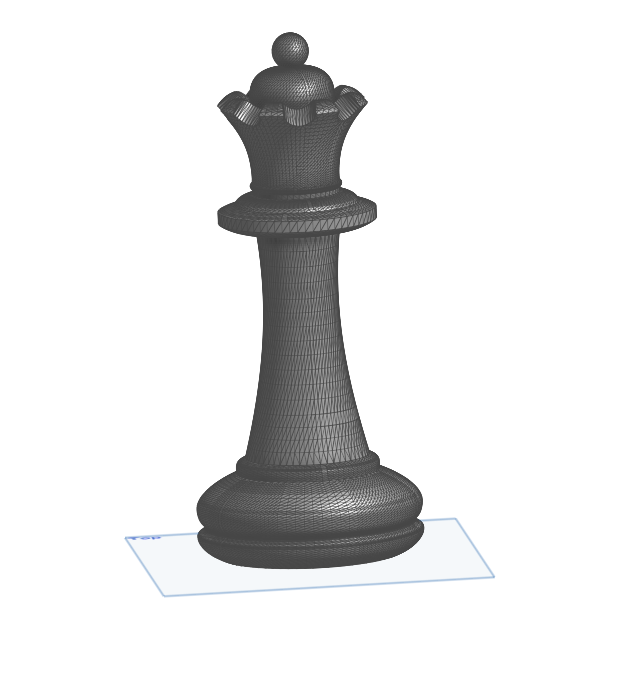
\includegraphics[width=0.15\textwidth]{./res/Schach/3D_Dame}
	\includegraphics[width=0.15\textwidth]{./res/Schach/3D_König}
	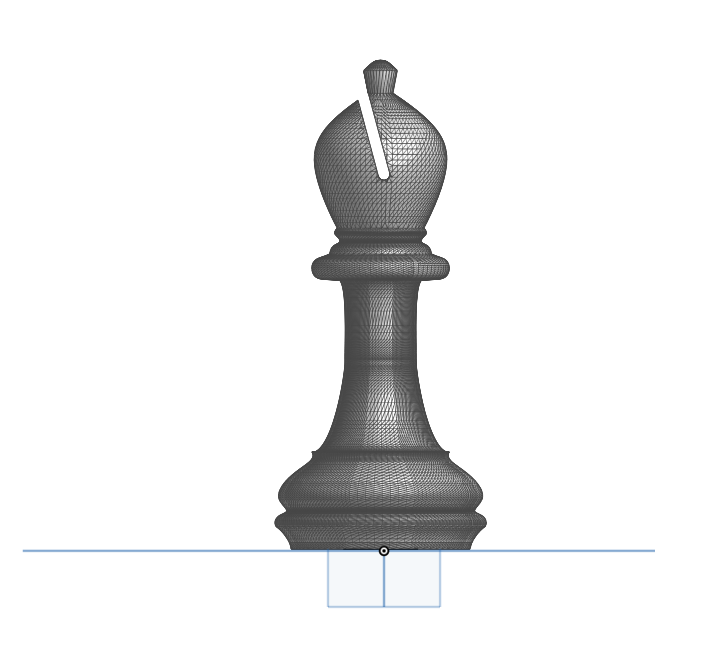
\includegraphics[width=0.15\textwidth]{./res/Schach/3D_Läufer}
	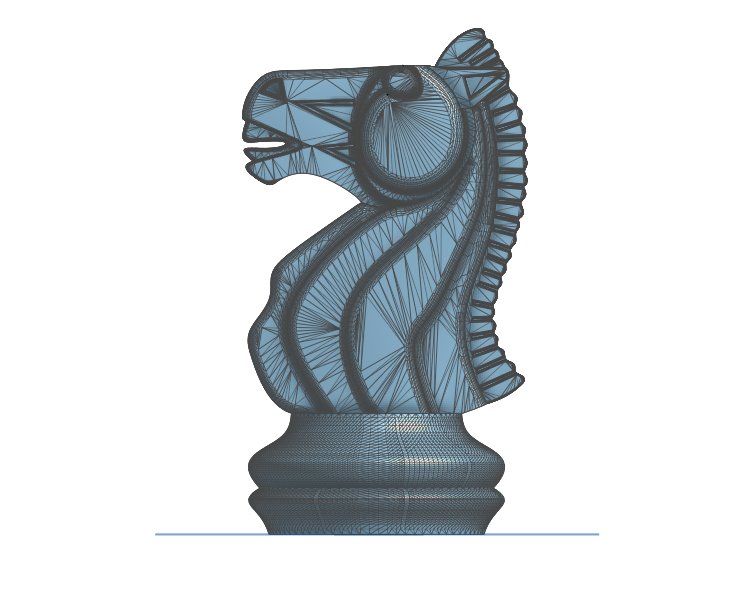
\includegraphics[width=0.15\textwidth]{./res/Schach/3D_Pferd}
	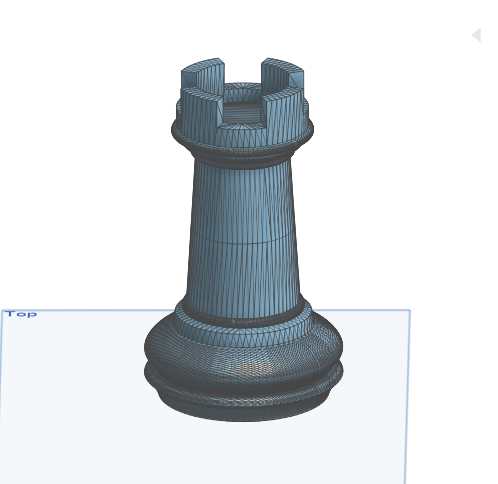
\includegraphics[width=0.15\textwidth]{./res/Schach/3D_Turm}
	\caption{3D-Modelle der Schachfiguren mit angepasster Befestigung für Magneten \cite{3D_Figuren}}
	\label{fig:3d_schachfiguren}
\end{figure}

\subsection{Softwarekonzeption des GUI}
Neben der Hardware musste auch eine Software entwickelt werden, die die erfassten Daten verarbeiten und visualisieren konnte. Da ich bereits Erfahrungen mit Java aus dem Unterricht hatte, entschied ich mich, die grafische Benutzeroberfläche (GUI) in dieser Sprache zu schreiben.\\
\\
Die Kommunikation zwischen dem Schachbrett und der Software sollte über eine serielle Schnittstelle erfolgen. Hierfür verwendete ich die Bibliothek \texttt{jSerialComm}\footcite{arduino_forum_java_serial}, die eine einfache Kommunikation mit dem Arduino ermöglichte. Der Arduino wiederum würde für das Auslesen der Hallsensoren verantwortlich sein und sendet die gesammelten Daten über die serielle Schnittstelle an die Java-Anwendung, wo sie weiterverarbeitet wurden. Zusätzlich nutzte ich die Bibliothek \texttt{jlayer-1.0.1}, um Soundeffekte in die Benutzeroberfläche zu integrieren.\footcite{youtube_Jlayer}\\
\\
Das Java-Projekt folgt einem modularen Aufbau und besteht aus mehreren zentralen Komponenten. Eine dieser Komponenten kümmert sich um die serielle Kommunikation, bei der die Bibliothek \texttt{jSerialComm} verwendet wird, um die Daten des Arduinos in Echtzeit zu empfangen. Ein weiteres Modul enthält die Schachlogik, die durch Klassen wie \texttt{ChessApp.java}, \texttt{Chessboard.java} und \texttt{ChessMove.java} den aktuellen Spielzustand verwaltet, Züge validiert und die Schachbrettposition speichert. Darüber hinaus wurden separate Klassen für die einzelnen Schachfiguren (z.B. \texttt{Pawn.java}, \texttt{Knight.java}, \texttt{Bishop.java} usw.) implementiert, die die spezifischen Zugregeln jeder Figur festlegen.\\
\\
Für die grafische Darstellung des Schachspiels werden die Java-Bibliotheken \textbf{AWT (Abstract Window Toolkit)} und \textbf{Swing} verwendet. AWT bietet grundlegende GUI-Komponenten wie Fenster, Buttons und Event-Handling, ist jedoch plattformabhängig. Swing, eine Erweiterung von AWT, nutzt hingegen plattformunabhängige Komponenten und ermöglicht anpassbare Oberflächen mit erweiterten Features wie \texttt{JPanel}, \texttt{JFrame} oder \texttt{JButton}. \\
\\
Die Klasse \texttt{GamePanel.java} erbt von \texttt{JPanel} und dient zur Visualisierung des Schachbretts. Sie überschreibt die \texttt{paintComponent}-Methode, um das Spielfeld mittels \texttt{Graphics2D} zu zeichnen (z.~B. Felder, Figuren). Mithilfe von \texttt{MouseListener} wird die Benutzerinteraktion (Klicken, Ziehen von Figuren) implementiert. Swing-Komponenten wie \texttt{JMenuBar} oder \texttt{JDialog} können zusätzlich Menüs oder Dialogfenster bereitstellen.\\
\\
Für die Audiowiedergabe (z.~B. Soundeffekte bei Zugausführung) kommt die Bibliothek \texttt{jlayer-1.0.1} zum Einsatz, die MP3-Dateien dekodieren kann.\footnote{\url{https://www.javazoom.net/javalayer/javalayer.html}} Die Integration erfolgt typischerweise über die Klasse \texttt{Player} aus dem Paket \texttt{javazoom.jl.player}.\\
\\
Ein Tutorial zur Grundlagenimplementierung eines Schachspiels in Java, das AWT/Swing und Objektorientierung erklärt, ist hier referenziert.\footnote{\url{https://example.com/chess-tutorial}} \\
\\
Zur Veranschaulichung der geplanten Softwarearchitektur habe ich ein UML-Diagramm erstellt, das den geplanten Ablauf des Projekts modelliert (siehe Abbildung~\ref{fig:uml_chess}). Das Diagramm wurde über den Verlauf des Projekts hinweg angepasst und zeigt, wie die verschiedenen Module in Beziehung zu einander stehen.\\
\begin{figure}[H]
	\centering
	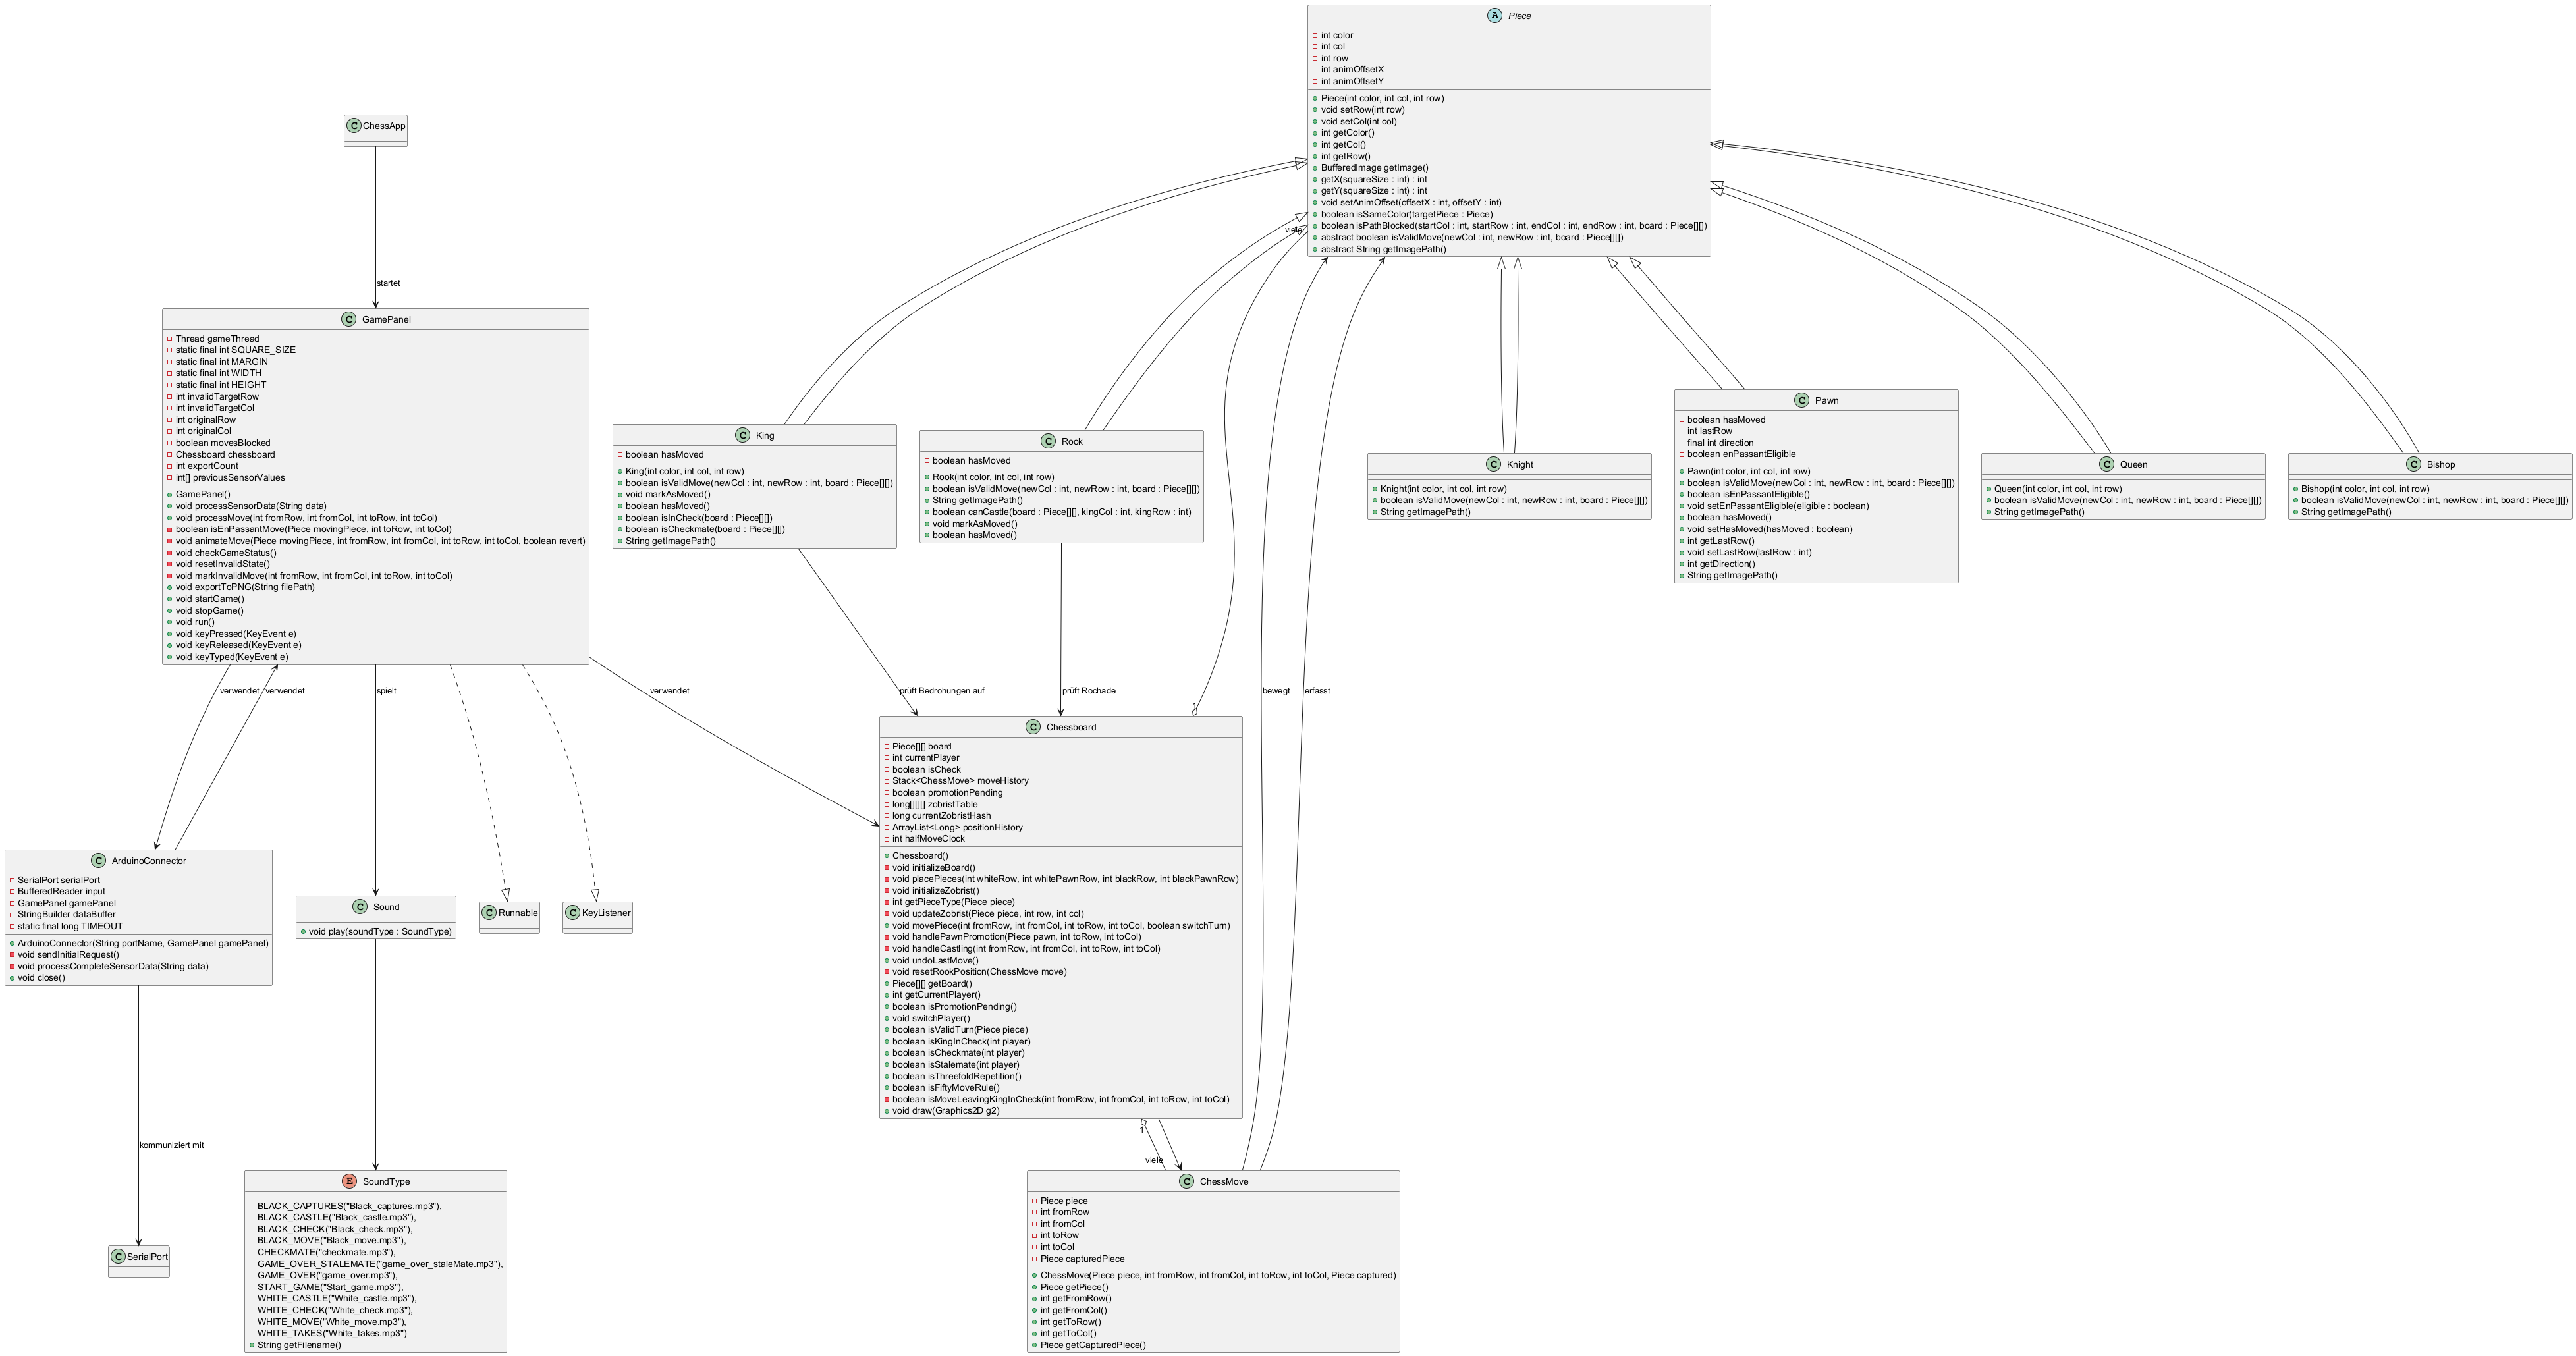
\includegraphics[width=1\textwidth, height= 0.8 \textheight]{./res/UML.png}
	\caption{UML-Diagramm der Softwarearchitektur}
	\label{fig:uml_chess}
\end{figure}
\newpage
\subsection{Konzeption der Sensordatenerfassung}
Die Grundidee der Sensordatenerfassung ist es, die Hallsensor-Matrix, die über einen Multiplexer angeschlossen ist, systematisch auszulesen und die erfassten Daten an die übergeordnete Software zu übermitteln, also dem GUI. Der Code aktiviert dabei in regelmäßigen Abständen jeweils einen Kanal des Multiplexers, liest den entsprechenden Sensorwert aus und überträgt diesen über die serielle Schnittstelle\\
\\
Konkret funktioniert dies so, dass der Arduino über vier Adressleitungen den gewünschten Kanal des Multiplexers auswählt. Sobald der jeweilige Hallsensor, der unter einem bestimmten Spielfeld platziert aktiviert wird, soll der Sensorwert ausgelesen und über einen Datenausgang ausgegeben werden. Dieser Wert zeigt an, ob ein Magnet (und damit eine Schachfigur) von dem Sensor erkannt wurde oder nicht. Anschließend wird dieser Wert zusammen mit der Kanalinformation (also der Position des Sensors auf dem Schachbrett) an die Java-Anwendung gesendet. Die Datenübertragung erfolgt über die serielle Schnittstelle, sodass die erfassten Informationen in Echtzeit verarbeitet und auf der grafischen Oberfläche angezeigt werden können.\\
\\
\subsection{Speicherung der Züge und Organisation der Historie}
Zu Beginn meiner Überlegungen zur Speicherung der Züge im Spiel zog ich in Erwägung, eine Liste zu verwenden – eine Datenstruktur, die sich besonders gut dafür eignet, alte Stellungen jederzeit erneut anzeigen zu können und dabei nur geringen Overhead mitbringt. Bei weiteren Recherchen stieß ich jedoch auf ein Video \footcite{zobrist_hashing_youtube}, in dem effiziente Methoden zur Organisation der Zughistorie im Schach vorgestellt wurden. Dort wurde ein Ansatz präsentiert, bei dem Züge mittels Zobrist-Hashing gespeichert werden – eine Methode, die den Spielzustand in kompakter Form abbildet.\\
\\
Der wesentliche Vorteil des Zobrist-Hashing-Ansatzes besteht darin, dass für jede mögliche Stellung auf dem Schachbrett ein eindeutiger Hash-Wert berechnet wird, der den aktuellen Zustand der Partie exakt widerspiegelt. Dies ermöglicht nicht nur eine schnelle und effiziente Speicherung, sondern auch einen zügigen Vergleich verschiedener Spielstände. Nach weiterer Recherche\footcite{wikipedia_zobrist} \footcite{Comptuerphile} entschied ich mich, diesen Ansatz in meinem Projekt zu integrieren, um die gesamte Historie der Schachpartie effizient zu verwalten und frühere Stellungen rasch überprüfen zu können.
%%%%
% Umsetzung und Implementierung
%%%%%
\section{Umsetzung und Implementierung}
\subsection{Hardwareentwicklung und Integration}
\label{sec:hardwareentwicklung}
Der erste Schritt bestand darin, das physische Schachbrett auszumessen, um die Maße eines Spielfeldes zu ermitteln. So konnte ich sicherstellen, dass die Sensoren exakt unter den vorgesehenen Feldern positioniert wurden.\\
\\
Unter jedem der 64 Felder platzierte ich Halssensoren, die den Zustand \glqq\textbf{HIGH}\grqq{} bzw. \glqq\textbf{LOW}\grqq{} melden, also ob eine Figur auf dem Feld ist oder nicht. Die Verkabelung erfolgte über zwei separate Breadboards, die jeweils die Stromversorgung für die rechte und linke Seite des Schachbretts übernahmen. Rote Kabel führten die Spannung (\SI{5}{\volt}), während schwarze Kabel als Ground dienten. Besonders aufwendig war das präzise Abisolieren und Anbringen der Kabel, da eine fehlerhafte Verkabelung zu unzuverlässigen Sensorwerten führen konnte.\\
\begin{figure}[H]
	\centering
	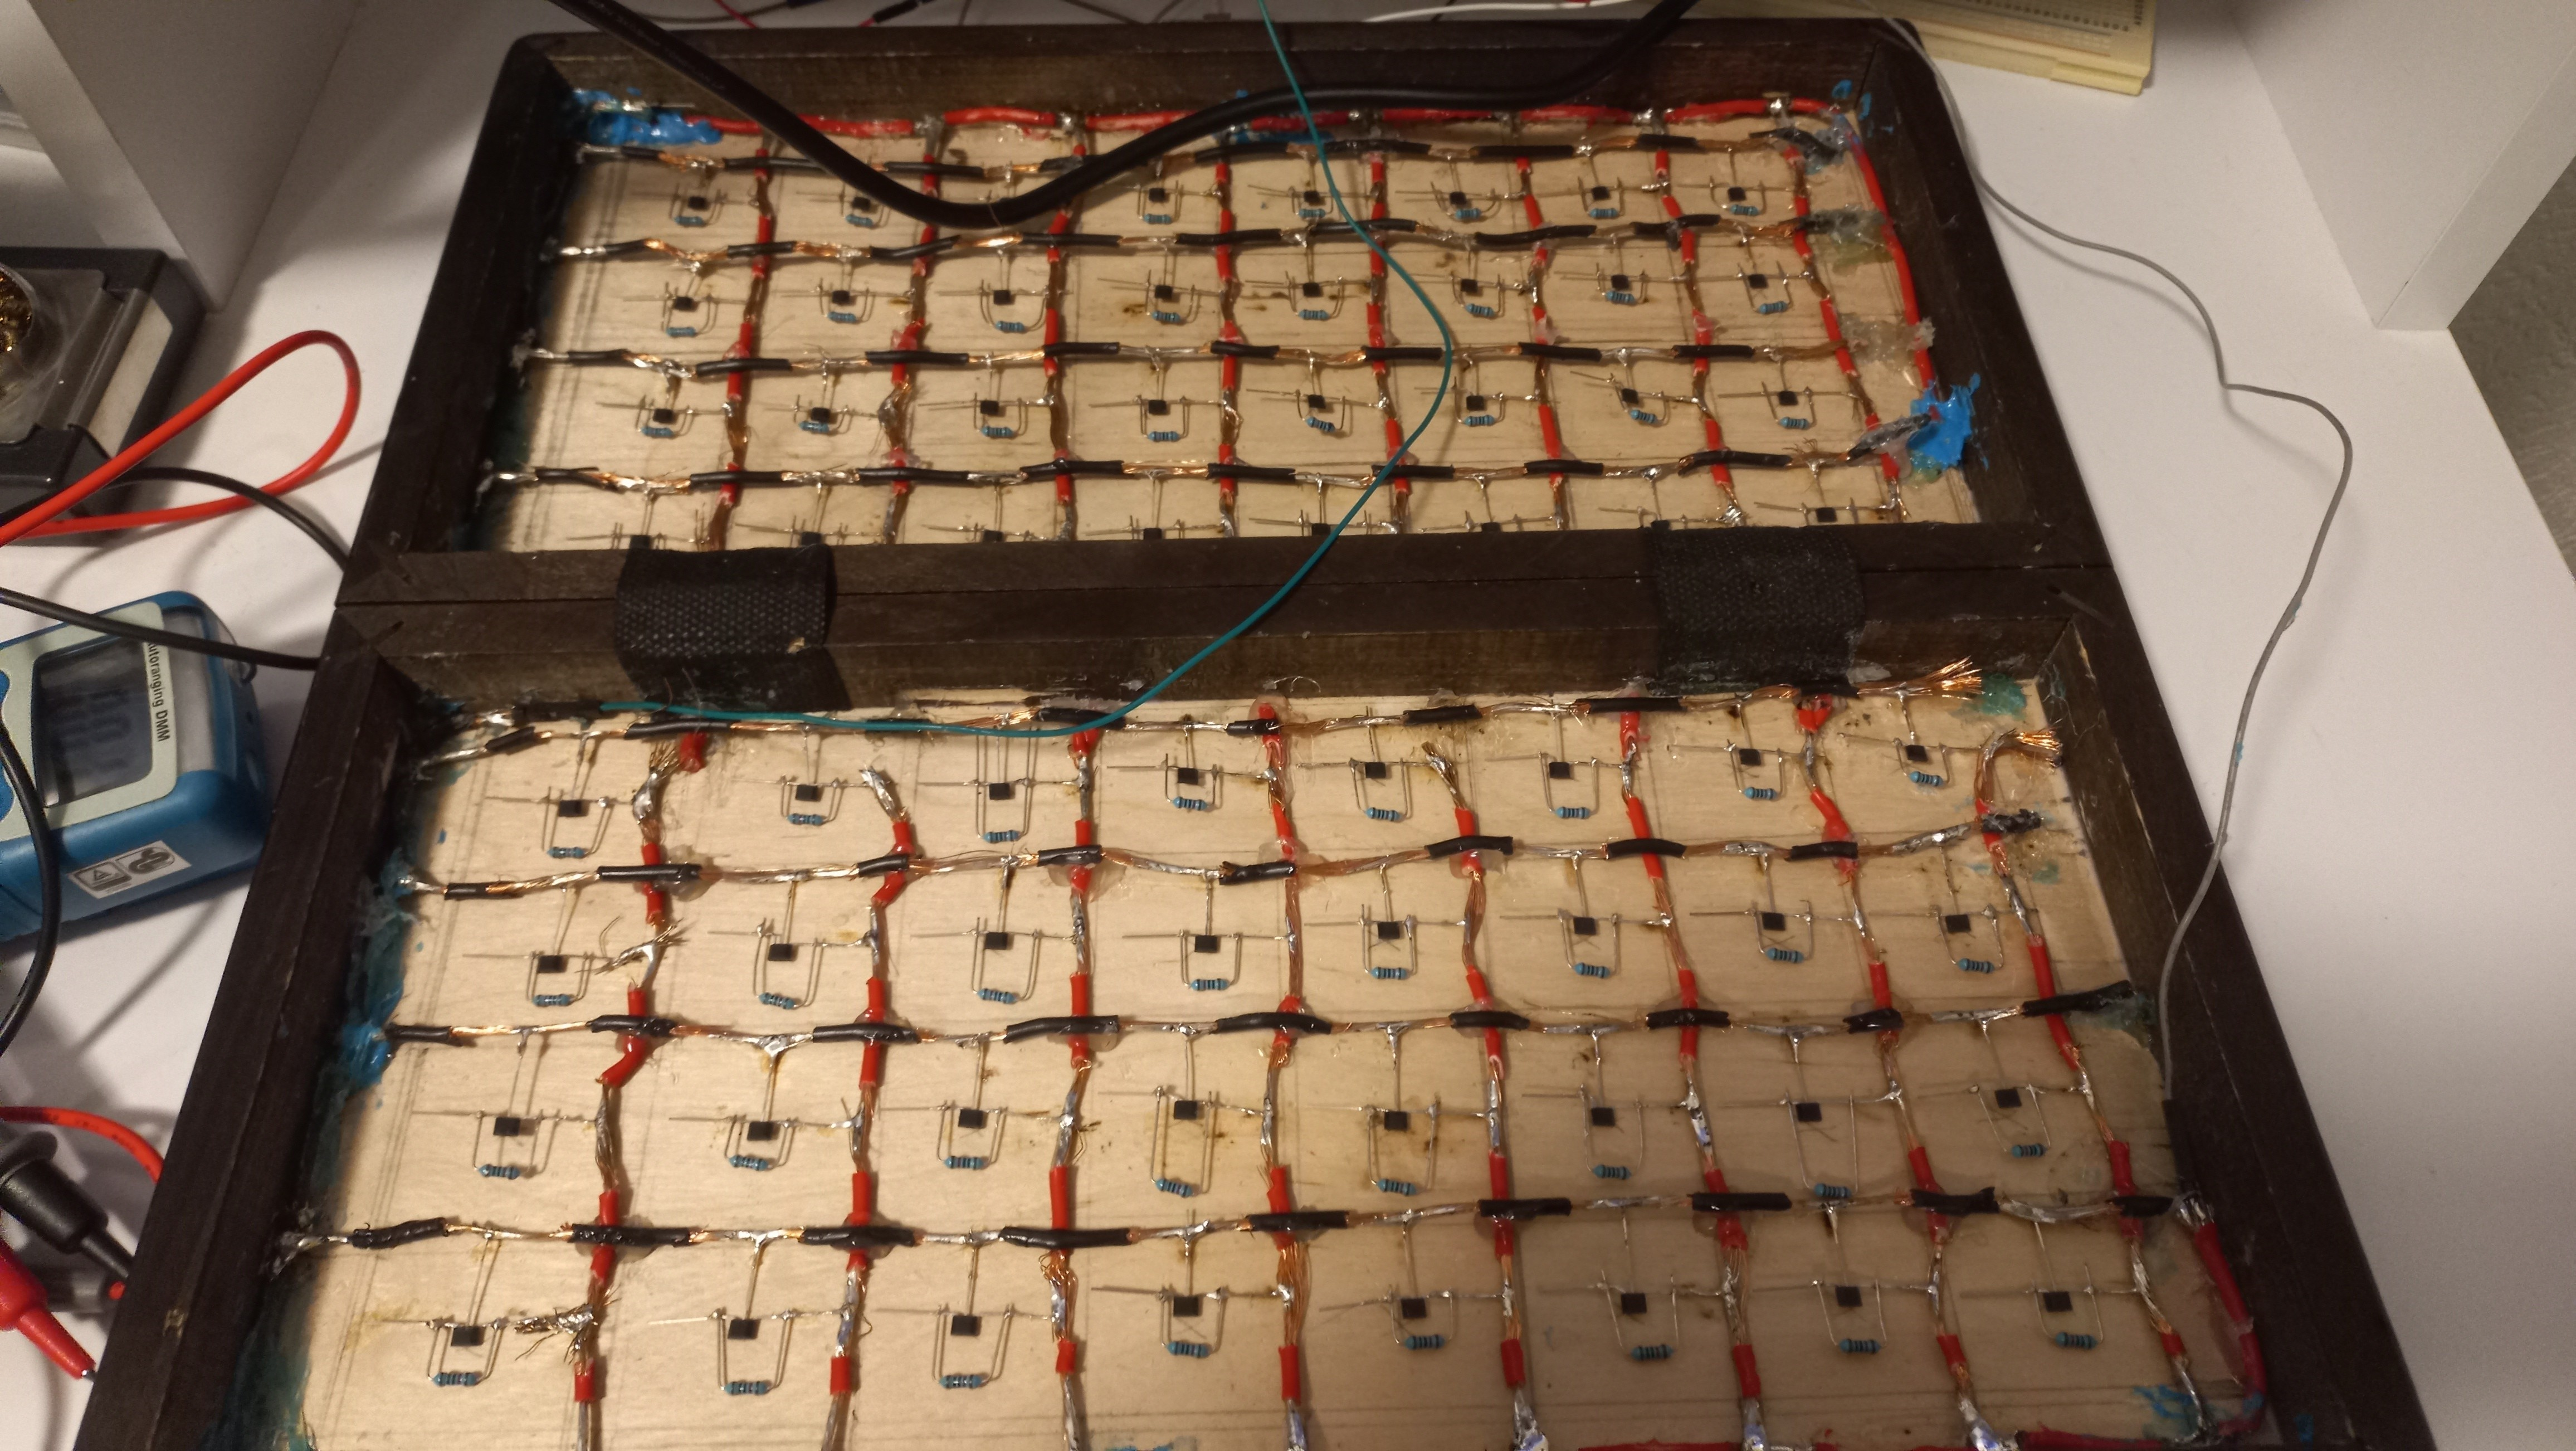
\includegraphics[width= 0.65\textwidth]{./res/Schachbrettgelötet.jpg}
	\caption{Vollendete Hallsensoren-Matrix}
	\label{fig: Schachbrett zuende gelötet}
\end{figure}
Wie zuvor geplant setzte ich beim auslesen der Sensor Daten MUX ein (siehe S.15), dabei musste ich sicherstellen, dass die 4-Bit-Steuercodes korrekt an die jeweiligen Pins des MUX übertragen wurden. Während des Aufbaus traten unerwartete Probleme auf: Zwei der eingesetzten MUX-Module waren defekt, was mich zwang, Ersatzkomponenten zu besorgen und die Schaltung anzupassen. Zudem wechselte ein MUX ständig unkontrolliert die Signale zwischen seinen Kanälen. Messungen ergaben, dass ein Kurzschluss zwischen den Leiterbahnen der Adressleitungen vorlag. Ein weiteres Problem war, dass eine der Adressleitungen „floating“ war, da die Lötstelle nicht richtig kontaktierte. Diese fehlerhafte Verbindung führte dazu, dass falsche Kanaladressen codiert wurden und somit falsche Sensorwerte übertragen wurden. Nach Behebung dieser Fehler verlötete ich die einzelnen Multiplexer Pins wieder richtig an und verkabelte dann die einzelnen Kanälen mit den Sensoren wie in Abbildung \ref{fig: SchachbrettundMUX} zu sehen ist:
\begin{figure}[H]
	\centering
	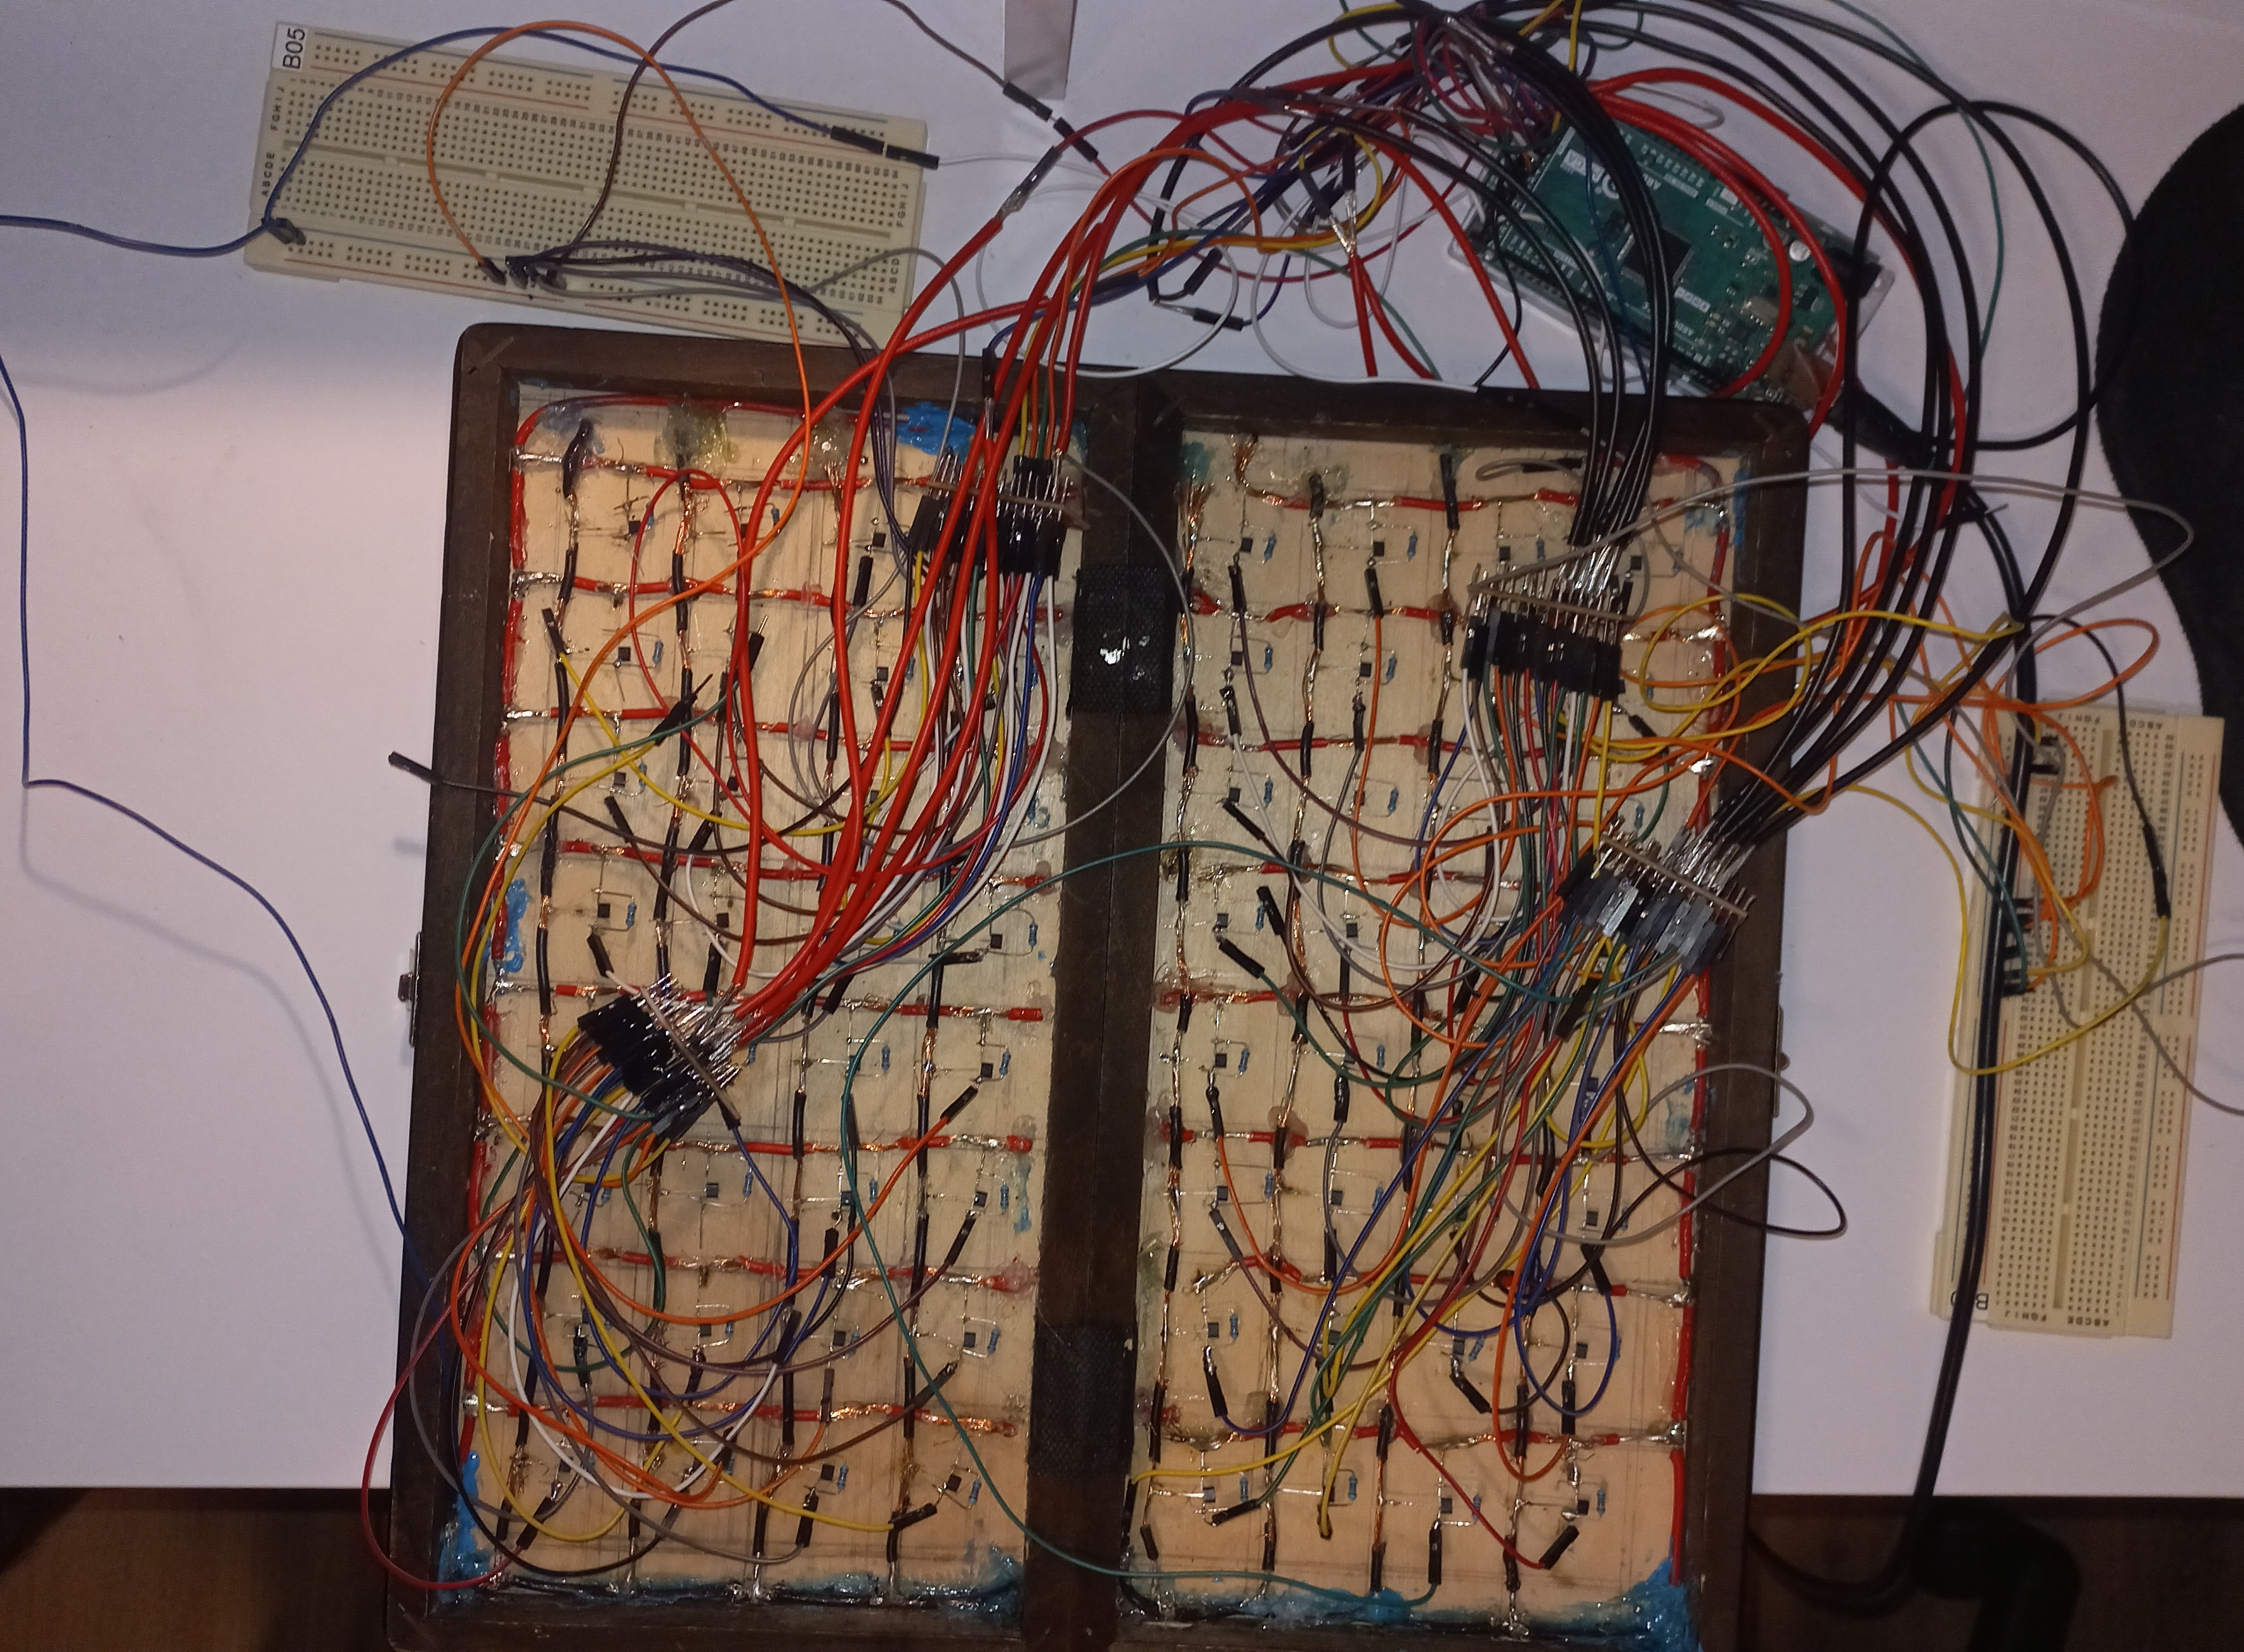
\includegraphics[width= 0.65 \textwidth]{./res/Muxdrangelötet.jpg}
	\caption{Vollendeter Prototyp der Schnittstelle}
	\label{fig: SchachbrettundMUX}
\end{figure}
\subsection{Mikrocontroller Logik}
Die Software Logik des Mikrocontrollers ist relativ simpel.
Zunächst wird ein zweidimensionales Array \texttt{muxPins} definiert, das für jeden der vier Multiplexer die zugehörigen Pin-Nummern enthält. Dabei werden die ersten vier Elemente eines jeden Arrays als Ausgänge zur Adressierung genutzt und das fünfte Element dient als Eingang für den Sensorsignalwert. Gleichzeitig wird ein Array \texttt{previousSensorValues} initialisiert, in dem die zuletzt gelesenen Sensorwerte gespeichert werden.\\
\\
\begin{lstlisting}[language=C, caption={Definition der Multiplexer-Pins und Initialisierung des Sensorwertspeichers}]
	int muxPins[4][5] = {
		{50, 51, 52, 53, 35},  // MUX1: Reihen 1-4, Spalten E-H
		{46, 47, 48, 49, 34},  // MUX2: Reihen 5-8, Spalten E-H
		{42, 43, 44, 45, 33},  // MUX3: Reihen 5-8, Spalten A-D
		{38, 39, 40, 41, 32}   // MUX4: Reihen 1-4, Spalten A-D
	};
	
	int previousSensorValues[64] = {0};
\end{lstlisting}

Im nächsten Schritt werden mehrere Hilfsfunktionen definiert. Die Funktion \texttt{setMuxChannel} wählt den gewünschten Kanal des Multiplexers aus, indem sie die digitalen Ausgänge entsprechend des Binärwerts des Kanal-Parameters setzt. Ein kurzes Delay stellt sicher, dass sich die Signale stabilisieren.\\
\\
\begin{lstlisting}[language=C, caption={Funktion \texttt{setMuxChannel} zur Kanalauswahl}]
	void setMuxChannel(const int sPins[4], int channel) {
		for (int i = 0; i < 4; i++) {
			digitalWrite(sPins[i], bitRead(channel, 3 - i));  // S3=LSB
		}
		delayMicroseconds(5);
	}
\end{lstlisting}

Die Funktion \texttt{readSensor} liest anschließend den Sensorsignalwert vom angegebenen Eingangspin aus. Dabei wird HIGH als 0 und LOW als 1 interpretiert, was in dieser Logik der Besetzungsstatus des Feldes ist.\\
\\
\begin{lstlisting}[language=C, caption={Funktion \texttt{readSensor} zum Auslesen des Sensorsignals}]
	int readSensor(int sigPin) {
		return digitalRead(sigPin) == HIGH ? 0 : 1;
	}
\end{lstlisting}

Um den aktuellen Zustand des Schachbretts über den Serial Monitor auszugeben, wird die Funktion \texttt{printBoard} verwendet. Diese gibt die 8x8-Anordnung als ASCII-Art aus, wobei besetzte Felder durch ein „X“ und leere Felder durch einen Punkt (".") dargestellt werden. Sie dient Hauptsächlich zum debuggen von möglicherweise auftretenden Problemen\\
\\
\begin{lstlisting}[language=C, caption={Funktion \texttt{printBoard} zur Darstellung des Schachbrettzustands}]
	void printBoard(int sensorValues[64]) {
		Serial.println("\nSchachbrett-Zustand:");
		Serial.println("  A B C D E F G H");
		Serial.println(" +----------------");
		for (int row = 0; row < 8; row++) {
			Serial.print(8 - row); // Zeilennummer
			Serial.print("|");
			for (int col = 0; col < 8; col++) {
				int index = row * 8 + col;
				Serial.print(sensorValues[index] ? "X " : ". "); // X = Figur, . = Leer
			}
			Serial.println();
		}
		Serial.println();
	}
\end{lstlisting}

Im \texttt{setup} werden der serielle Anschluss initialisiert und alle benötigten Pins der Multiplexer als Ausgänge (für die Kanalauswahl) bzw. als Eingang (für das Sensorsignal) konfiguriert. Der Arduino gibt anschließend eine Bestätigung über den Serial Monitor aus.\\
\\
\begin{lstlisting}[language=C, caption={Setup-Funktion im Arduino-Code}]
	void setup() {
		Serial.begin(115200);
		Serial.println("Starte Setup...");
		
		for (int mux = 0; mux < 4; mux++) {
			for (int i = 0; i < 4; i++) {
				pinMode(muxPins[mux][i], OUTPUT);
			}
			pinMode(muxPins[mux][4], INPUT);
		}
		
		Serial.println("Setup abgeschlossen!");
	}
\end{lstlisting}

In der \texttt{loop}-Funktion erfolgt die kontinuierliche Überwachung des Schachbretts. Zunächst werden alle 64 Sensorwerte ausgelesen, indem für jeden Multiplexer alle 16 Kanäle sequenziell aktiviert und der Sensorsignalwert abgefragt wird. Die Position des Sensors wird dabei anhand berechneter Zeilen- und Spaltenindizes ermittelt und im Array \texttt{sensorValues} abgelegt.\\
\\
Nach dem Auslesen erfolgt ein Vergleich der aktuellen Sensorwerte mit den vorherigen Werten. Wird genau an zwei Stellen ein Unterschied festgestellt – ein Feld, das von \glqq besetzt \grqq zu \glqq leer \grqq wechselt, und ein Feld, das von \glqq leer \grqq zu \glqq besetzt \grqq wechselt –, so wird dies als gültiger Zug interpretiert. Der erkannte Zug wird dann in einem vorgegebenen Format (eingeleitet mit \texttt{START,} und abgeschlossen mit \texttt{(,END)} über den Serial-Port ausgegeben. Abschließend werden die aktuellen Sensorwerte in das Array \texttt{previousSensorValues} kopiert, sodass der nächste Durchlauf den neuen Zustand als Referenz verwendet wird. Ein Delay von 500 Millisekunden den einzelnen Zyklen gewährleistet eine stabile Abtastrate.\\
\\
\begin{lstlisting}[language=C, caption={Die \texttt{loop}-Funktion zur Erfassung und Übertragung der Sensorwerte}]
	void loop() {
		int sensorValues[64] = {0};
		
		// Sensordaten auslesen
		for (int mux = 0; mux < 4; mux++) {
			for (int channel = 0; channel < 16; channel++) {
				setMuxChannel(muxPins[mux], channel);
				int val = readSensor(muxPins[mux][4]);
				
				// Positionsberechnung
				int reihe = (mux < 2) ? (channel / 4) : 4 + (channel / 4);
				int spalte = (mux % 2 == 0) ? (7 - (channel % 4)) : (3 - (channel % 4));
				int index = reihe * 8 + spalte;
				
				sensorValues[index] = val;
			}
		}
		
		// Schachbrett mit aktuellen Sensorwerten ausgeben zum Debugen
		printBoard(sensorValues);
		
		// Bewegungserkennung: Vergleiche aktuelle Sensorwerte mit den vorherigen
		int fromIndex = -1, toIndex = -1, diffCount = 0;
		for (int i = 0; i < 64; i++) {
			if (sensorValues[i] != previousSensorValues[i]) {
				diffCount++;
				if (previousSensorValues[i] == 1) {
					fromIndex = i;
				} else {
					toIndex = i;
				}
			}
		}
		
		// Sende nur Zugdaten im erwarteten Format, wenn genau zwei Unterschiede festgestellt wurden
		if (diffCount == 2 && fromIndex != -1 && toIndex != -1) {
			Serial.print("Erkannter Zug: ");
			Serial.print((fromIndex / 8) + 1);
			Serial.print((char)('A' + (fromIndex % 8)));
			Serial.print(" -> ");
			Serial.print((toIndex / 8) + 1);
			Serial.print((char)('A' + (toIndex % 8)));
			Serial.println();
			
			Serial.print("START,");
			Serial.print((fromIndex / 8) + 1);  
			Serial.print(",");
			Serial.print((char)('A' + (fromIndex % 8))); 
			Serial.print(",");
			Serial.print((toIndex / 8) + 1);
			Serial.print(",");
			Serial.print((char)('A' + (toIndex % 8)));
			Serial.println(",END");
		}
		
		// Sensorwerte aktualisieren
		memcpy(previousSensorValues, sensorValues, sizeof(previousSensorValues));
		delay(500);
	}
\end{lstlisting}


\subsection{Implementierung des GUI}
\label{sec:softwareentwicklung}

In der \texttt{Chessboard}-Klasse wird die gesamte Schachlogik umgesetzt – angefangen bei der Anfangsaufstellung der Figuren bis hin zur Validierung von Sonderzügen wie Rochade, En Passant und Bauernumwandlung. In der Methode \texttt{movePiece} wird ein Zug ausgeführt, wobei zunächst geprüft wird, ob es sich um einen Spezialfall wie En Passant handelt. Anschließend wird der Zug in der internen Brettdarstellung durchgeführt, wobei der Zobrist-Hash zur schnellen Erkennung von Stellungshistorien aktualisiert wird. Gleichzeitig wird der Zug in der \texttt{moveHistory} gespeichert, sodass er später beispielsweise für die \texttt{undoLastMove}-Funktion verwendet werden kann.

\begin{lstlisting}[language=Java, caption={Auszug aus \texttt{movePiece} in der \texttt{Chessboard}-Klasse}]
	public void movePiece(int fromRow, int fromCol, int toRow, int toCol, boolean switchTurn) {
		Piece movingPiece = board[fromRow][fromCol];
		Piece captured = board[toRow][toCol];
		
		// En Passant: Bei diagonalem Zug eines Bauern in ein leeres Feld
		if (movingPiece instanceof Pawn && Math.abs(toCol - fromCol) == 1 && board[toRow][toCol] == null) {
			int capturedPawnRow = fromRow;
			captured = board[capturedPawnRow][toCol];
			updateZobrist(captured, capturedPawnRow, toCol);
			board[capturedPawnRow][toCol] = null;
		}
		
		// Entferne die Figur von der alten Position aus dem Hash
		updateZobrist(movingPiece, fromRow, fromCol);
		if (captured != null) {
			updateZobrist(captured, toRow, toCol);
		}
		// Speichere den Zug in der Historie
		moveHistory.push(new ChessMove(movingPiece, fromRow, fromCol, toRow, toCol, captured));
		// Fuehre den Zug aus
		board[toRow][toCol] = movingPiece;
		board[fromRow][fromCol] = null;
		
		// Aktualisiere den Hash der neuen Stellung
		updateZobrist(movingPiece, toRow, toCol);
		
		// Sonderlogik: Bauernumwandlung und Rochade
		if (movingPiece instanceof Pawn) {
			handlePawnPromotion(movingPiece, toRow, toCol);
		}
		if (movingPiece instanceof King && Math.abs(toCol - fromCol) == 2) {
			handleCastling(fromRow, fromCol, toRow, toCol);
		}
		
		// Spielerwechsel und weitere Statusupdates
		if (switchTurn) {
			switchPlayer();
		}
	}
\end{lstlisting}

Das \texttt{GamePanel} steuert die Anzeige und Animation der Züge. In der Methode \texttt{processMove} wird zunächst sichergestellt, dass Züge momentan verarbeitet werden dürfen. Anschließend wird geprüft, ob sich an der Startposition tatsächlich eine Figur befindet. Ist dies der Fall, wird die Gültigkeit des Zugs überprüft, bevor bei einem gültigen Zug eine Animation gestartet und bei einem ungültigen Zug der Zielbereich rot markiert sowie eine Rückanimation ausgeführt wird.

\begin{lstlisting}[language=Java, caption={Auszug aus der \texttt{processMove}-Methode in \texttt{GamePanel}}]
	public void processMove(int fromRow, int fromCol, int toRow, int toCol) {
		// Blockierung, falls Züge momentan nicht erlaubt sind
		if (movesBlocked || chessboard.isPromotionPending()) {
			System.out.println("Zug wird momentan nicht verarbeitet.");
			return;
		}
		
		Piece movingPiece = chessboard.getBoard()[fromRow][fromCol];
		if (movingPiece == null) {
			System.out.println("Keine Figur an der Startposition!");
			resetInvalidState();
			repaint();
			return;
		}
		
		// Prüfung, ob der Zug gültig ist (eigene Figur, regelkonforme Bewegung, etc.)
		if (!movingPiece.isValidMove(toCol, toRow, chessboard.getBoard())) {
			markInvalidMove(fromRow, fromCol, toRow, toCol);
			animateMove(movingPiece, fromRow, fromCol, toRow, toCol, true);
			return;
		}
		
		// Animation und Soundausgabe bei gültigem Zug
		animateMove(movingPiece, fromRow, fromCol, toRow, toCol, false);
	}
\end{lstlisting}

Die Kommunikation mit dem Arduino erfolgt über die \texttt{jSerialComm}-Bibliothek. Ein Datenlistener wird eingerichtet, der die eintreffenden Sensordaten in einen Puffer schreibt und erst verarbeitet, wenn ein vollständiger Nachrichtenblock (zwischen \texttt{START} und \texttt{END}) empfangen wurde. Sobald ein solcher Block vorliegt, wird dieser an die Methode \texttt{processCompleteSensorData} weitergeleitet und der Puffer zurückgesetzt.

\begin{lstlisting}[language=Java, caption={Auszug aus der \texttt{serialEvent}-Methode in \texttt{ArduinoConnector}}]
	serialPort.addDataListener(new SerialPortDataListener() {
		@Override
		public int getListeningEvents() {
			return SerialPort.LISTENING_EVENT_DATA_AVAILABLE;
		}
		
		@Override
		public void serialEvent(SerialPortEvent event) {
			if (event.getEventType() == SerialPort.LISTENING_EVENT_DATA_AVAILABLE) {
				try {
					String line = input.readLine();
					if (line == null) {
						return;
					}
					
					dataBuffer.append(line);
					
					if (dataBuffer.indexOf("START,") >= 0 && dataBuffer.indexOf(",END") >= 0) {
						int startIndex = dataBuffer.indexOf("START,");
						int endIndex = dataBuffer.indexOf(",END") + 4;
						String completeMessage = dataBuffer.substring(startIndex, endIndex);
						processCompleteSensorData(completeMessage);
						
						dataBuffer.delete(0, endIndex);
					}
				} catch (Exception e) {
					e.printStackTrace();
				}
			}
		}
	});
\end{lstlisting}

Über die Methode \texttt{processSensorData} in der \texttt{GamePanel}-Klasse werden die vom Arduino empfangenen Daten interpretiert. Diese Methode erwartet einen String im Format „START, <v0>,<v1>\,...,<v63>, END“ und validiert zunächst das Format. Nach dem Entfernen der Start- und Endmarkierungen wird der String anhand von Kommas in einzelne Werte zerlegt. Es werden genau vier Werte erwartet, die dann in interne Koordinaten umgerechnet werden, bevor der Schachzug über die Methode \texttt{processMove} verarbeitet wird.

\begin{lstlisting}[language=Java, caption={Codeausschnitt: Verarbeitung der Sensordaten}]
	/**
	* Verarbeitet die vom Arduino empfangenen Daten.
	* Erwartet wird ein String im Format:
	* "START,<v0>,<v1>,...,<v63>,END"
	* 
	* Bei genau vier Werten wird ein Zug angenommen.
	*
	* @param data Die empfangenen Daten als String.
	*/
	public void processSensorData(String data) {
		data = data.trim();
		
		// Validiere das Datenformat
		if (!data.startsWith("START,") || !data.endsWith(",END")) {
			System.out.println("Ungueltiges Datenformat: " + data);
			return;
		}
		
		// Entferne "START," und ",END"
		String inner = data.substring(6, data.length() - 4);
		String[] parts = inner.split(",");
		
		// Erwarte 4 Werte: FromRow, FromCol, ToRow, ToCol
		if (parts.length != 4) {
			System.out.println("Erwartet 4 Werte (FromRow,FromCol,ToRow,ToCol), erhalten: " + parts.length);
			return;
		}
		
		try {
			// Konvertiere die Werte in Integer
			int fromRow = Integer.parseInt(parts[0].trim());
			int fromCol = parts[1].trim().charAt(0) - 'A'; // Spalte A=0, B=1, etc.
			int toRow = Integer.parseInt(parts[2].trim());
			int toCol = parts[3].trim().charAt(0) - 'A';
			
			// Konvertiere visuelle Reihen (1-8) in interne Reihen (0-7)
			int internalFromRow = 8 - fromRow;
			int internalToRow = 8 - toRow;
			
			// Verarbeite den Zug
			processMove(internalFromRow, fromCol, internalToRow, toCol);
			
		} catch (NumberFormatException | StringIndexOutOfBoundsException e) {
			System.err.println("Fehler beim Parsen der Zugdaten: " + e.getMessage());
		}
	}
\end{lstlisting}

Die \texttt{ChessMove}-Klasse dient zur Dokumentation einzelner Züge. Jedes Objekt dieser Klasse enthält alle wichtigen Informationen zum Zug, wie Start- und Zielposition sowie eine eventuell geschlagene Figur. Mit dieser Klasse wird jeder Zug in der Zughistorie gespeichert, was unter anderem für Funktionen wie das Rückgängigmachen von Zügen genutzt wird. Dadurch kann die Schnittstelle eine genaue Historie der Partie erstellen.

\begin{lstlisting}[language=Java, caption={Auszug aus der \texttt{ChessMove}-Klasse}]
	public class ChessMove {
		private Piece piece;
		private int fromRow, fromCol;
		private int toRow, toCol;
		private Piece capturedPiece;
		
		public ChessMove(Piece piece, int fromRow, int fromCol, int toRow, int toCol, Piece captured) {
			this.piece = piece;
			this.fromRow = fromRow;
			this.fromCol = fromCol;
			this.toRow = toRow;
			this.toCol = toCol;
			this.capturedPiece = captured;
		}
		
		// Getter-Methoden...
	}
\end{lstlisting}

Der Zobrist-Hash wird in der \texttt{Chessboard}-Klasse verwendet, um die Stellung des Schachbretts effizient zu repräsentieren und zu vergleichen. Hierbei wird für jede mögliche Kombination aus Farbe, Figurentyp und Position ein zufälliger Wert generiert. Der Gesamt-Hash der Stellung wird dann durch das bitweise XOR ( \texttt{\^} ) der entsprechenden Werte aller auf dem Brett befindlichen Figuren berechnet. Bei einem Zug wird der Hash durch erneutes XORen der Werte der betroffenen Positionen aktualisiert. Dadurch können Änderungen schnell und effizient vorgenommen werden, und alte Stellungen werden in einer Historie gespeichert, um beispielsweise Wiederholungen zu erkennen.

\begin{lstlisting}[language=Java, caption={Auszug aus der Zobrist-Initialisierung in \texttt{Chessboard}}]
	private void initializeZobrist() {
		Random rand = new Random();
		zobristTable = new long[2][6][MAX_ROW * MAX_COL];
		for (int color = 0; color < 2; color++) {
			for (int type = 0; type < 6; type++) {
				for (int pos = 0; pos < MAX_ROW * MAX_COL; pos++) {
					zobristTable[color][type][pos] = rand.nextLong();
				}
			}
		}
	}
\end{lstlisting}

Neben der Initialisierung existieren zwei wesentliche Methoden, die den Zobrist-Hash während des Spiels aktualisieren. Die Methode \texttt{updateZobrist} aktualisiert den aktuellen Zobrist-Hash, indem sie den Einfluss einer bestimmten Figur an einer bestimmten Position toggelt. Dabei wird zunächst überprüft, ob das übergebene Figurenobjekt \texttt{null} ist. Falls nicht, wird der Typ der Figur mittels \texttt{getPieceType(piece)} ermittelt und die Position linear als \texttt{pos = row * MAX\_COL + col} berechnet. Anschließend wird der aktuelle Hash-Wert durch eine bitweise XOR-Operation mit dem Wert aus der vorinitialisierten \texttt{zobristTable} an der entsprechenden Stelle aktualisiert. Durch dieses Verfahren wird der Einfluss der Figur an der betreffenden Position entweder hinzugefügt oder entfernt, wobei bei doppelter Anwendung der ursprüngliche Zustand wiederhergestellt wird.

\begin{lstlisting}[language=Java, caption={Methode \texttt{updateZobrist}}]
	private void updateZobrist(Piece piece, int row, int col) {
		if (piece == null) return;
		int type = getPieceType(piece);
		int pos = row * MAX_COL + col;
		currentZobristHash ^= zobristTable[piece.getColor()][type][pos];
	}
\end{lstlisting}

Die Methode \texttt{undoLastMove} macht den letzten Zug rückgängig und stellt sowohl das Brett als auch den Zobrist-Hash in den Zustand vor dem Zug zurück. Zunächst wird geprüft, ob die Zughistorie nicht leer ist. Falls ein Zug vorhanden ist, wird dieser mittels \texttt{pop()} entfernt und in einer Variablen gespeichert. Anschließend wird der Hash am Zielort des Zuges aktualisiert, um den Beitrag der Figur an dieser Position zu entfernen. Danach erfolgt die Rücksetzung des Zugs auf dem Brett: Die Figur wird an ihre ursprüngliche Position zurückgesetzt und eine eventuell geschlagene Figur wiederhergestellt. Der Hash wird daraufhin erneut aktualisiert, um den Einfluss der Figur an ihrem Ursprungsort hinzuzufügen, und falls eine Figur geschlagen wurde, wird deren Hash-Beitrag ebenfalls wieder eingerechnet. Abschließend wird die interne Position der Figur korrigiert, und bei speziellen Zügen wie der Rochade wird durch Aufruf von \texttt{resetRookPosition(lastMove)} auch der Turm an die korrekte Position zurückgesetzt. Zum Schluss erfolgt ein Wechsel des aktiven Spielers.

\begin{lstlisting}[language=Java, caption={Methode \texttt{undoLastMove}}]
	public void undoLastMove() {
		if (!moveHistory.isEmpty()) {
			ChessMove lastMove = moveHistory.pop();
			updateZobrist(lastMove.getPiece(), lastMove.getToRow(), lastMove.getToCol());
			board[lastMove.getFromRow()][lastMove.getFromCol()] = lastMove.getPiece();
			board[lastMove.getToRow()][lastMove.getToCol()] = lastMove.getCapturedPiece();
			updateZobrist(lastMove.getPiece(), lastMove.getFromRow(), lastMove.getFromCol());
			if (lastMove.getCapturedPiece() != null) {
				updateZobrist(lastMove.getCapturedPiece(), lastMove.getToRow(), lastMove.getToCol());
			}
			lastMove.getPiece().setRow(lastMove.getFromRow());
			lastMove.getPiece().setCol(lastMove.getFromCol());
			if (lastMove.getPiece() instanceof King && Math.abs(lastMove.getToCol() - lastMove.getFromCol()) == 2) {
				resetRookPosition(lastMove);
			}
			switchPlayer();
		}
	}
\end{lstlisting}
%%%%%
% Evaluation und Test
%%%%%
\section{Evaluation und Test}
\label{sec:evaluation}
\subsection{Test der Hardwarekomponenten}
\label{sec:fehleranalyse}
Nach dem ersten Aufbau der Mensch-Maschine-Schnittstelle traten einige unerwartete Probleme auf. Insbesondere die MUX wiesen Fehlfunktionen auf. Ein erster Fehler bestand darin, dass ein MUX ständig Signale vertauschte, sodass die Eingaben nicht korrekt übermittelt wurden. Zur systematischen Fehlersuche wurde die \texttt{printBoard}-Methode eingesetzt, um den aktuellen Zustand der Sensoren visuell darzustellen und fehlerhafte Signalverteilungen zu identifizieren. Nach einigen Tests und Messungen stellte sich heraus, dass ein Kurzschluss zwischen den Leiterbahnen der Adressleitungen der beiden Kanäle des MUX bestand. Dies führte dazu, dass sich die beiden Kanäle gegenseitig beeinflussten und falsche Signale erzeugt wurden. Zur Überprüfung der Leiterbahnen wurden kontinuierlich Widerstände zwischen den Pins gemessen, um Kurzschlüsse oder Unterbrechungen frühzeitig zu erkennen.\\
\\
Ein Problem war auch, dass ein MUX eine ständige „Signalverwirrung“ aufwies, indem mehrere Kanäle immer einen HIGH Output zurückgaben, selbst wenn nur ein einzelner Sensor aktiviert war. Dieser Fehler konnte dadurch behoben werden, dass festgestellt wurde, dass eine der Adressleitungen „floating“ war. Das bedeutete, dass diese Leitung keine stabile Verbindung aufwies und die Verbindung zur Platine nicht korrekt hergestellt war, was zu einem dauerhaften LOW, also einem 0-Bit in der Schaltabelle des MUX, führte und das Signal verfälschte. Zusätzlich wurden bei der Überprüfung der Messwerte und Spannungen mehrere physisch beschädigte Sensoren entdeckt, deren Widerstandswerte außerhalb der Toleranz lagen. Diese Sensoren wurden daraufhin ausgetauscht, um eine zuverlässige Signalübertragung zu gewährleisten. Nachdem diese Fehler behoben und die Lötstellen überprüft sowie korrekt angesetzt wurden, funktionierte der MUX wieder stabil.\\
\\
Ein weiteres Problem trat auf, als mehrere Sensoren gleichzeitig ein Output-Signal von sich gaben, obwohl nur ein Sensor einen Input bekommen hatte. Dieser Fehler konnte durch eine genauere Prüfung der Platine gelöst werden, da die MUX und die Sensoren durch eine fehlerhafte Verbindung zwischen den Adressleitungen einen Kurzschluss hatten und nicht korrekt funktionierten. Bei der Analyse zeigten sich zudem sporadisch schwache Magnet-Signale einzelner Felder, die auf mangelnden Kontakt oder unzureichende Magnetstärke zurückzuführen waren. Durch Justieren der Magnetpositionen und Nachlöten kritischer Verbindungen wurde dieses Problem reduziert.\\
\\
\subsection{Test der Softwarekomponenten}
\label{sec:softwaretest}
Die größte Herausforderung in den Softwaretests lag in der korrekten Handhabung der Spiellogik, insbesondere bei Sonderzügen wie der Rochade. Die für die Validierung und Ausführung der Züge zuständige \texttt{processMove}-Methode funktionierte zwar für die meisten regulären Züge, stieß jedoch bei komplexeren Manövern wiederholt auf Probleme. Ein initialer Logikfehler führte dazu, dass das Spielbrett aus der falschen Perspektive interpretiert wurde – bei weißen Zügen reagierte die Software fälschlicherweise aus Sicht von Schwarz. Dies äußerte sich in inkonsistenten Zugvalidierungen und wurde durch eine fehlerhafte Koordinatenzuordnung im Code verursacht. Durch gezieltes Debugging der Board-Repräsentation konnte dieser Fehler lokalisiert und durch Korrektur der Indexberechnungen behoben werden.\\
\\
Besonders die Rochade bereitete Schwierigkeiten, da ihre Bedingungen nicht immer zuverlässig erkannt wurden, was zu fehlerhaften Spielverläufen führte. Ein zentrales Problem zeigte sich darin, dass bei einem fehlerhaft ausgeführten Zug die Schnittstelle alle weiteren Züge blockierte. Dabei verstand die Software lediglich, dass eine Bewegung stattgefunden hatte, und bewertete den folgenden Zug als ungültig, selbst wenn im realen Spielverlauf eine Korrektur, wie das Zurücksetzen eines Bauern um einen Schritt, vorgenommen wurde. Dieses Verhalten führt dazu, dass manche Fälle, in denen Züge zwar korrigiert, aber von der Software nicht erkannt werden, die Rückverfolgung und Korrektur erheblich erschweren. Zudem traten sporadisch Probleme bei der Erkennung von Zügen auf, wenn Magnet-Signale aufgrund von Positionierungsungenauigkeiten oder Materialschwächen zu schwach ausfielen. Durch eine Anpassung der Signalverarbeitung, einschließlich einer dynamischen Schwellwertanpassung, konnte die Robustheit der Zugerkennung signifikant\\ verbessert werden.

\subsection{Bewertung und Zusammenfassung der Testergebnisse}
\label{sec:bewertung}

Das entwickelte System zur Digitalisierung von Schachzügen hat seine Kernfunktion – die Erfassung und Darstellung von Spielzügen – grundsätzlich erfolgreich umgesetzt. Die Tests zeigen jedoch sowohl Stärken als auch Grenzen des Prototyps, die im Folgenden zusammengefasst werden.\\
\\
Die größten Erfolge liegen in der gelungenen Hardware-Software-Integration. Nach der Behebung anfänglicher Probleme wie Kurzschlüssen in den Adressleitungen oder lose gelöteten Sensoren konnte das System Standardzüge zuverlässig erkennen. Bewegungen von Bauern, Läufern oder Springern wurden in den meisten Fällen korrekt digitalisiert und in der grafischen Benutzeroberfläche angezeigt. Die selbst programmierte Software übersetzte die erfassten Daten erfolgreich in eine digitale Partienotation, was besonders für Trainingszwecke oder Partieanalysen nützlich ist. Die Fehlerbehebung mithilfe des Multimeters und der \texttt{printBoard}-Methode erwies sich als effektiv, um Hardwareprobleme systematisch zu isolieren und zu beheben.\\
\\
Allerdings traten Herausforderungen bei komplexeren Anforderungen auf. Sonderzüge wie die Rochade oder der „en passant“-Schlag bereiteten der Software anfangs Schwierigkeiten, da die Implementierung der Schachregeln nicht alle Randfälle abdeckte. Erst durch mehrfache Überarbeitung des Codes – etwa die Korrektur der Koordinatenindizes und die Verbesserung der Validierungslogik – konnten diese Züge zuverlässiger erkannt werden. Ein weiterer kritischer Punkt war die mechanische Empfindlichkeit der Hardware: Leicht verschobene Sensoren führten zu Fehldetektionen. Dies erfordert in der Praxis sorgfältiges Positionieren der Figuren, was das Spielerlebnis beeinträchtigen kann.\\
\\
Die Stabilität des Systems erwies sich als zweischneidig. Zwar arbeitete die Hardware nach Abschluss aller Reparaturen stabil, doch die manuellen Nachjustierungen (z. B. Nachlöten von Kontakten) zeigten, dass das Design für den Dauereinsatz noch zu anfällig ist. Auch die Software zeigte Schwächen bei der Fehlerrückverfolgung: Wurde ein Zug physisch korrigiert (z. B. durch Zurücksetzen einer Figur), erkannte das System dies nicht immer automatisch, was zu Schwierigkeiten im Spielfluss führt\\
\\
Zusammenfassend lässt sich sagen, dass der Prototyp alle grundlegenden Anforderungen eines digitalen Schachbretts erfüllt, aber noch nicht ausgereift ist. Die Stärken liegen in der kostengünstigen Umsetzung und der gelungenen Verbindung von analogem Spielgefühl mit digitaler Darstellung. Die Schwächen – vor allem die eingeschränkte Regelabdeckung und mechanische Sensibilität – verdeutlichen, warum professionelle Lösungen komplexer und teurer sind. Für ein Schulprojekt ist das Ergebnis dennoch ein trotz Problemen ein Erfolg.
\section{Zusammenfassung und Ausblick}
\label{sec:zusammenfassung_und_ausblick}
Im Rahmen dieses Projekts wurde ein Schachbrett entwickelt, das in der Lage ist, Spielzüge automatisch zu erfassen und digital zu verarbeiten. Zu Beginn stand die Idee im Fokus, eine Mensch-Maschine-Schnittstelle zu schaffen, die analoge Schachzüge mit minimalem externem Eingriff erkennt. Dafür wurden unter den einzelnen Feldern Magnetsensoren platziert, um zuverlässig zu detektieren, ob ein Feld besetzt ist oder nicht.\\
\\
die Schnittstelle war in der Lage, viele Standardzüge korrekt zu erkennen und den Spielverlauf digital zu speichern. Insbesondere für einfache Zugfolgen funktionierte das Prinzip zuverlässig. Dennoch traten mit zunehmender Spieldauer Probleme auf: Sonderzüge wie Rochade oder Bauernumwandlungen führten zu Fehlinterpretationen, und die Fehleranfälligkeit der Schnittstelle nahm zu. Besonders problematisch war die fehlende Möglichkeit, Schachfiguren eindeutig zu unterscheiden. Dies erschwerte die Korrektur fehlerhafter Züge erheblich, da die Schnittstelle nicht nachvollziehen konnte, welche Figur ursprünglich an einer bestimmten Position stand. Fehlerhafte Erkennungen summierten sich dadurch im Verlauf der Partie, was letztlich zu Diskrepanzen zwischen der digitalen Spiellogik und der realen Brettstellung führte. \\
\\
Trotz dieser Herausforderungen war das Projekt eine äußerst lehrreiche Erfahrung. Die Entwicklung einer eigenen Hardware-Lösung und deren Integration in eine Software war ein faszinierender Prozess, bei dem zahlreiche technische und konzeptionelle Herausforderungen bewältigt werden mussten. Ich konnte wertvolle Erkenntnisse über die Signalverarbeitung von Sensoren, Störsignale in elektronischen Schaltungen sowie die komplexen Wechselwirkungen zwischen Hardware und Software gewinnen. Besonders spannend war es zu beobachten, wie eine physische Aktion – das Bewegen einer Schachfigur – in einem digitalen System abgebildet wurde. Auch wenn nicht alle Aspekte der Schnittstelle reibungslos funktionierten, war es ein beeindruckender Moment, wenn ein korrekt erkannter Zug auf dem Bildschirm dargestellt wurde.\\  
\\
Dieses Projekt war ein wichtiger Prototyp, der als Grundlage für zukünftige Iterationen dienen kann. Ein zentrales Ziel zukünftiger Versionen wäre die Implementierung der Figurenidentifikation, um eine zuverlässigere Fehlerkorrektur zu ermöglichen. Dafür könnten verschiedene Ansätze in Betracht gezogen werden.
\\
Ein weiterer interessanter Ansatz zur Verbesserung der Spielvalidierung wäre der Einbau von Elektromagneten in die Felder des Schachbretts. Diese könnten Figuren bei Bedarf magnetisch fixieren, um illegale Züge sofort zu korrigieren. Wenn ein Spieler versucht, eine Figur entgegen den Schachregeln zu bewegen, würde das System die Magnetkraft aktivieren und die Figur am ursprünglichen Feld halten. Gleichzeitig könnte ein solches System verhindern, dass Spieler außerhalb ihrer Zugzeit Figuren bewegen – die Magnete wären nur für den aktiven Spieler deaktiviert. Dies würde nicht nur regelwidrige Züge blockieren, sondern auch das Spieltempo verbessern, indem versehentliches Verschieben von Figuren während der Denkpause unterbunden wird.\\
\\
Für die Fehlerkorrektur ließe sich dieses Konzept erweitern: Bei Erkennung eines ungültigen Zuges durch die Software könnten die Magnete automatisch reaktiviert werden, um die Figur in ihre Ausgangsposition zurückzuzwingen. Kombiniert mit einer visuellen Warnung auf dem digitalen Interface entstünde so ein robustes Fehlerfeedback-System. Die Hardware-Implementierung würde allerdings neue Herausforderungen mit sich bringen, etwa die präzise Ansteuerung von 64 Einzelmagneten und die Integration in die bestehende Sensorik.\\
\\
Ein weiterer sinnvoller Zusatz wäre die Möglichkeit, gespeicherte Spielstände später fortzusetzen. Durch die Archivierung von Brettstellungen in einer Datenbank könnten Nutzer gezielt Schlüsselmomente einer Partie speichern – etwa komplexe Mittelspielpositionen oder Endspielszenarien –, um diese zu Trainingszwecken erneut aufzurufen. Ambitionierte Spieler hätten so die Chance, Alternativzüge zu testen oder Fehler retrospektiv zu analysieren. Praktisch ließe sich dies sogar auf unterbrochene Partien erweitern. Während diese Funktionalität den Rahmen der aktuellen Implementierung überschreitet, würde sie das Schachbrett zu einem flexiblen Lernwerkzeug machen. \\
\\
Zusammenfassend hat mir dieses Projekt nicht nur wertvolle technische Erkenntnisse vermittelt, sondern auch gezeigt, dass Fehler und unerwartete Herausforderungen essenzielle Bestandteile des Entwicklungsprozesses sind. Die kontinuierliche Verbesserung eines Systems durch iterative Optimierung ist ein spannender und lohnender Prozess. Trotz der bestehenden Herausforderungen hat mir die Arbeit an dieser Mensch-Maschine-Schnittstelle große Freude bereitet, und ich sehe in der Weiterentwicklung dieser Idee viel Potenzial für zukünftige Projekte.  

\newpage
	\section{Quellenverzeichnis}
	\printbibliography[title = Quellen]
	\newpage
	\listoffigures 
\end{document}